\documentclass{sig-alternate}
\usepackage{graphicx}
\usepackage{blindtext}
\usepackage{url}
\usepackage{listings}
\usepackage{fancyvrb}
\usepackage{float}
\usepackage{hyperref}


\begin{document}
\title{BaseFS -\\ Basically Available, Soft State, Eventually Consistent Filesystem for Cloud Management}
\numberofauthors{1} %  in this sample file, there are a *total*
\author{
\alignauthor
Marc Aymerich Gubern\\
    \affaddr{Universitat Politecnica de Catalunya UPC}\\
    \email{marc.aymerich@est.fib.upc.edu}
}
\additionalauthors{}
\date{30 July 1999}

\maketitle

\begin{abstract}
BaseFS is a peer-to-peer distributed filesystem for cloud configuration, designed to operate under the network conditions and administrative requirements commonly found on Wireless Community Networks. Nodes do not need to trust each other, the core data-structure is an append-only Merkle DAG with monotonic and cryptographic properties that allows for efficient and secure verification of data sent by untrusted nodes. Decentralized write permission is achieve using a hierarchy-based public key infrastructure built into the Merkle DAG, allowing for automatic resolution of write conflicts based on \textit{proof-of-authority}. Finally, a gossip layer is used for disseminate changes very quickly and efficiently as well as for maintaining group membership in an scalable way. With no single point-of-failure, BaseFS can provide levels of availability, scalability and performance never seen before on a cloud configuration tool.

\end{abstract}
\section{Introduction}
%significance of the topic
One of the steps towards building a successful distributed system is establishing effective configuration management. It is a complex engineering process responsible for planning, identifying, tracking and verifying changes in the software and its configuration as well as maintaining configuration integrity throughout the life cycle of the system \cite{Yermolaiev:managing}.

Some successful tools exist to aid in this process, e.g. Chef and Puppet only to name a few. In these solutions, the system configuration is written in recipes that converge every few minutes. While this approach works well for static configuration, it fails to provide an ideal solution for more dynamic state, where a near real-time convergence is desirable. Because of the need for faster provisioning, elasticity in cloud environments or quickly respond to failures, systems like Zookeeper, etcd or Consul, that target this very specific problem, have emerged. They are distributed key-value stores designed for keeping the global state of the system. We can make a rough distinction between the \textit{static configuration management} tasks solved by tools like Chef or Puppet and the \textit{dynamic configuration management} commonly solved by key-value stores like Zookeeper, etcd or Consul.

Existing \textit{dynamic configuration management} solutions are designed with strong consistency models and client-server architectures. They have server nodes that require a quorum of nodes to operate (usually a simple majority). They choose consistency over availability under the face of a network partition. Design decisions based on the assumption that these systems are deployed on a data center-like environment. Where machines are homogeneous, with predictable performance, connected by fast networks, with low churn and operated by a team of highly skilled engineers, while all being part of a single administrative domain. But these assumptions are not always true.

Community cloud computing\cite{marinos2009community} is an emerging model where infrastructure is built using a collaborative effort. It is often the result of individual users providing spare resources to a common pool. As we can imagine the set of constrains faced by this kind of distributed systems are different from those we can find in the typical data center. Hardware is heterogeneous, it tends to be consumer-grade with higher failure rates and lower performance. Resources range in quantity and quality from one node to another. Nodes enter and leave the system more often. The network might be slow and unreliable; partitions may occur more frequently. The administrative boundary between organizations is sometimes blurry, with requirements for a decentralized administration of the infrastructure. Limitations on the technical capacity for effectively deploying and managing complex distributed systems may also exist, since the operators are sometimes members of the community that volunteer their time, but with limited SLA commitment. In short, community cloud architecture is peer-to-peer\cite{babaoglupeer, ranjan2010peer}, in contrast to the centralized model of traditional clouds.

The main contribution of this thesis is to provide a novel approach to solve cloud configuration management problems on a decentralized, more networked constrain, environments. First we present a case for a more available and less consistent configuration management solution. Then, we introduce the design an implementation of BaseFS, an eventually consistent gossip-style distributed filesystem specifically designed for cloud and configuration management. Experimental results from a prototype implementation are presented in section \ref{evaluation} and finally we reflect on the future of BaseFS.

\section{Background}

Zookeeper, etcd and Consul are consolidated distributed key-value stores for shared configuration and service discovery. But they present limitations in the context of community cloud. The more relevant, and the ones we hope to address, are: a) geographical and administrative scalability, b) trading consistency over availability and c) deployment complexities.

\subsection{Scalability Limits}

Existing work rely on fault-tolerant, distributed coordination algorithms like Paxos\cite{lamport2001paxos} and Raft\cite{ongaro2014search} are used because of their strong consistency properties. But coordinated consensus is expensive, processes can't make progress independently: a majority of nodes have to agree on every decision first. Constant communication between nodes is needed, making the system hard to scale beyond small clusters or across wide-area networks. 
Coordination algorithms are notoriously hard to implement\cite{ongaro2014search}, and even harder to make them tolerate Byzantine failures. In the end, nodes need to trust each other, making it hard to scale as the number of administrative domains increases. The real scalability challenges faced by community cloud computing are not about the size of the system, but on \textbf{geographic} and \textbf{administrative} scalability.

By removing coordinated consensus, geographic scalability improves naturally, as progress is no longer restricted by network delay anymore. On the other hand, administrative scalability can be improved by removing the need for nodes having to trust each other. 

\subsection{Availability Under Network Partition}

The CAP theorem is a valid and useful tool for reasoning about fundamental trade-offs made on the design of a distributed system\cite{brewer2012cap}, although it has recently been the subject of scrutiny and debate regarding whether it is overstated or not\cite{Kleppmann:CAP}. The acronym stands for:

\begin{itemize}
\item Consistency: all nodes see the same data at the same time
\item Availability: node failures do not prevent survivors from continuing
\item Partition tolerance: the system continues to operate despite message loss due to network failure
\end{itemize}
    
The theorem states that a distributed system facing a network partition has to choose between staying available or being consistent. In our case all the current solutions err on the side of consistency. These solutions are commonly called CP (Consistent but not available under Partition). The main implication is that in case of partition nodes under a minority partition will not be able to make progress.

CP systems are a fragile and complex piece of the infrastructure, and making a system depend on them makes progress impossible for minority partitions. It is important to stress that consistency presented by the CAP theorem actually refers to \textbf{strong consistency}. This consistency definition can be relaxed and allow availability and some kind of consistency less than "all nodes see the same data at the same time". A typical example is eventual consistency, which guarantees that after some undefined amount of time all replicas will converge on the same value.

Cheap wireless links is the network infrastructure of choice for some community cloud deployments. Nodes continuously entering and leaving the system are also expected. With unstable quorums, latency, packet loss, low bandwidth and network partitions a CP system deployed on these conditions will have a hard time staying available and deliver good performance. In this situation a cloud management solution that \textbf{focuses on availability} while at the same time provides a low conflict rate, fast convergence, and low divergence time will be desirable.


\subsection{Complexity}

Existing configuration management solutions are complex to deploy and maintain. They need dedicated quorum servers that have to be protected from untrusted parties. Extra efforts need to be placed on making sure network partitions do not occur, the entire system's availability may depend on it. The use of non-standardized APIs that operators need to learn also increases its complexity. Networked APIs such as REST or RPC don't come for free, applications need to account for network error conditions and optimize for IO overhead.

Additionally, because these tools are designed with data center conditions in mind, they have to be tunned to operate across wide area networks. Meaning, securing communications with a VPN and increasing the \textit{consensus timeouts}, a performance sensitive parameter which by default is very low.

While all this complexity has not been a problem for corporations with in-house teams of well paid, highly skilled, engineers, Community cloud is sometimes build and operated by volunteers, and there is not always good incentives for investing large amounts of effort into solving complex technical problems.

Complexity can be lowered by removing the need for dedicated servers and make the system P2P. Without a single point-of-failure nor the need for nodes to trust each other, some of the main attributes that led Bittorrent to achieve massive adoption. On the other hand, a filesystem API is something developers are already familiar with, and all programming languages have libraries for.

\subsection{Existing P2P Filesystems}

Before reinventing the wheel with a new solution, we examine if existing P2P filesystems can be used for effective cloud management.

Syncthing and other P2P-based Dropbox-like applications are discarded because trust between nodes is assumed by means of a shared secret. Additionally, Syncthing dissemination model is based on periodic state synchronization, a bad model for fast dissemination of highly dynamic content.

IPFS, short for InterPlanetary File System, is a peer-to-peer hypermedia protocol, addressed by content and identities\cite{IPFS}. At the time of this writing IPFS lacks update notification, applications have to actively fetch updates for content they are interested in. A polling model for data that changes frequently is not scalable. Another issue is the \textit{single-point of contention} of its Merkle DAG design. IPFS uses a Merkle DAG inspired on GIT, changes are linked by the \textit{commit tree}, effectively creating a \textit{single-point-of-conflict} for the whole filesystem. Simultaneous changes on \textbf{different files} cause conflict (branches), seriously limiting concurrent writes scalability. For a version control system having all related changes linked together by a commit tree is desirable, but for an application that allows concurrent writes from multiple nodes a \textit{per-file point-of-conflict} is more desirable. 


\section{Design and Implementation}

BaseFS builds on top of ideas and concepts coming from existing technologies used by successful distributed systems that have been developed over the last decade or so. The inspiration from BaseFS comes from Bitcoin, Serf, IPFS and Consul, just to name a few. In this section we present the main design aspects of our prototype implementation, including:

\begin{enumerate}
\item \textbf{Log} - a Merkle DAG of content-addressed immutable entries. Described in \ref{log}
\item \textbf{View} - provides a conflict free composition of the log entries. Described in \ref{view}
\item \textbf{Network} - maintains membership, manages connections to other peers, uses various underlying network protocols. Described in \ref{network}
\item \textbf{Filesystem} - emulates filesystem operations on \textit{view} operations. Described in \ref{filesystem}.
\item \textbf{Modules Overview} - how everything is glued together. Described in \ref{modules}
\end{enumerate}

\subsection{Log}  \label{log}

BaseFS \textit{log} is composed by two types of hash addressable objects:

\begin{itemize}
    \item Log entries - Nodes of a Merkle DAG containing the whole history of log operations
    \item Log blocks - File content chunks
\end{itemize}


\paragraph{Log entries}
BaseFS log entries contain all the filesystem metadata (or i-nodes) organized as an add-only monotonic Merkle DAG, with the convenience of also being CvRDT \textit{Convergent Replicated Data Type}\cite{shapiro2011comprehensive}.

A Merkle DAG is a directed acyclic graph whose objects are linked to each other by their hash. As illustrated in figure \ref{fig:log}, log entries (representing files, directories, links...) are linked to their parent directory, conforming to the hierarchy of the filesystem. Using cryptographic hashes has many useful properties:

\begin{itemize}
\item Content addressing: all content is uniquely identified by its SHA-224 hash checksum.
\item Tamper resistance: all content is verified with its hash.
\item Deduplication: all objects that hold the exact same content are equal, and only stored once.
\item Casual ordering: the object linked is older than the object itself, hashes can not be calculated in advance.
\end{itemize}


\begin{figure}
\centering
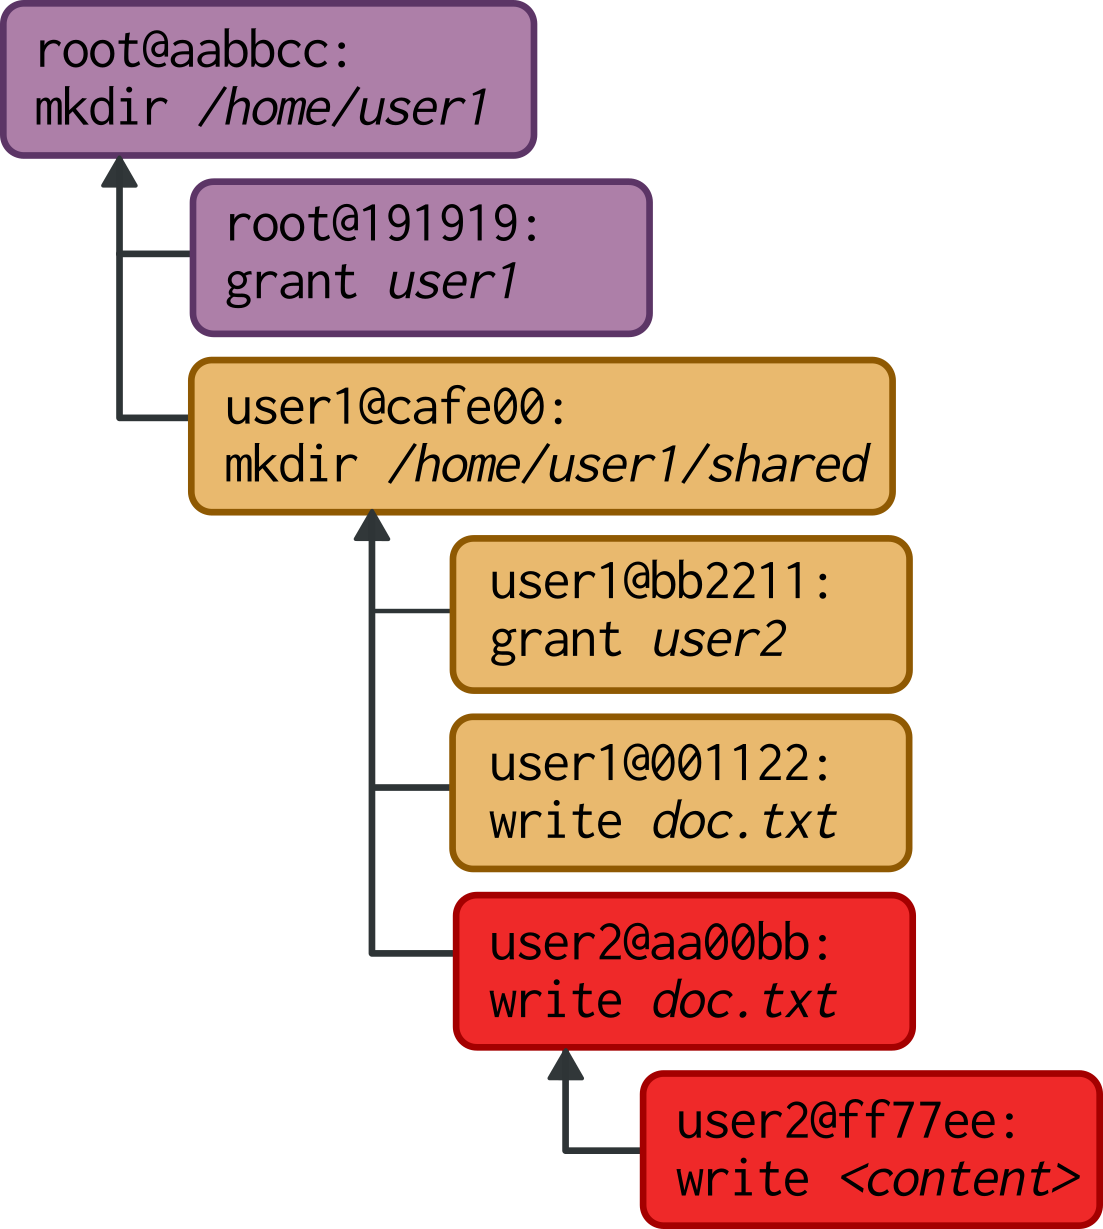
\includegraphics[width=150pt]{imgs/log.png}
\caption{Partial log representation}
\label{fig:log}
\end{figure}

Log entries also satisfy the definition of \textit{Convergent Replicated Data Type}. A semilattice, partially ordered set that has a join with a \textit{least upper bound}, with sufficient conditions:

\begin{itemize}
 \item a) Associativity $f(f(a, b), c) = f(a, f(b, c))$
 \item b) Commutativity $f(a, b) = f(b, a)$
 \item c) Idempotency $f(f(a)) = f(a)$
\end{itemize}

Conditions that allow for a gossip-style week communication channel with message loss, out of order, or multiple delivery. The only required condition is eventual delivery. If two nodes see the same events, they are on the same state. Characteristic known as strong eventual consistency (SEC). Under the constraints of the CAP theorem, CvRDT provide the strongest consistency guarantees for AP settings\cite{Wikipedia:CRDT}.

The specifications for the log entry fields are the following:

\begin{enumerate}
\item \textbf{Prent hash} - SHA-224 hash hexdigest of the target entry. 
\item \textbf{Timestamp} - a UNIX timestamp that represents the time at which the log entry was created. BaseFS does not provide any mechanism to validate this timestamp with a global clock, this field is purely informative used for example by \texttt{ls} command.
\item \textbf{Action} - filesystem operations needed for enabling all the common requirements for a cloud configuration tool
    \begin{itemize}
    \item \texttt{mkdir}: make a new directory
    \item \texttt{write}: create or update a file content
    \item \texttt{delete}: deletes an entry
    \item \texttt{revert}: reverts a path to some previous state
    \item \texttt{grant}: enables write permissions to specific key
    \item \texttt{revoke}: disables write permissions for an specific key
    \item \texttt{ack}: acknowledge a log branch as valid, needed for maintaining state after key granting or revocation.
    \item \texttt{link}: a hard link between two entries
    \item \texttt{slink}: a symbolic link pointing to some path
    \item \texttt{mode}: give or remove executable file permissions
    \end{itemize}

remove operations are implemented with \texttt{delete} and \texttt{link} actions
\item \textbf{Name} - determines the name of the directory, file, link or key. Like UNIX file names, BaseFS name size is limited to 256 characters. Paths are constructed using these names.
\item \textbf{Size} - size of the file in bytes. This is a performance optimization because computing the whole file size every time an ls is performed is really expensive.
\item \textbf{Content} - depending on the action, the log entry content may contain:
    \begin{itemize}
    \item \texttt{write}: SHA-224 hexdigest of the first block content
    \item \texttt{grant} or \texttt{revoke}: Base64 encoded EC public key
    \item \texttt{slink}: target path, could be any path, not restricted to BaseFS filesystem.
    \item \texttt{link} and \texttt{revert}: target entry hexdigest SHA-224 hash
    \item \texttt{mode}: mode value
    \end{itemize}
\item \textbf{Key fingerprint} - The public key fingerprint used to sign the log entry.
\item \textbf{Signature} - base64 encoding of the entry's signature. Elliptic curve cryptography is used for the smaller size of the keys compared to equivalent RSA security level.
\end{enumerate}

Notice that version control is provided naturally by the monotonic and immutability properties of BaseFS Merkle DAG. All history is available, \texttt{revert} entries only need to reference a previous entry hash for the path state to be reverted.

\paragraph{Write Permissions}

\texttt{grant} and \texttt{revoke} entries are used for directory-based permission management. A \texttt{grant} entry gives a public key permissions to write into a directory and all its sub-directories. Since all log entries are authenticated by its author signature, BaseFS nodes are able to identify and ignore log entries that do not satisfy this rule. 

BaseFS is a self-certified filesystem, a trust chain can be built only by trusting the filesystem root key, owned by the node that first bootstrapped the filesystem.

Special considerations are needed when revoking keys. The user doing the revocation must acknowledge (\texttt{ACK} entry) all related leaf entries, otherwise leaf entries with a now invalid key will be ignored.


\paragraph{Log blocks}

File content is divided into chunks called blocks. As represented in figure \ref{fig:blocs}, blocks form a hashed linked list. A log entry points to the first block, and each block references the next block by its hash. An empty hash is used to signal end of content.

\begin{figure}
\centering
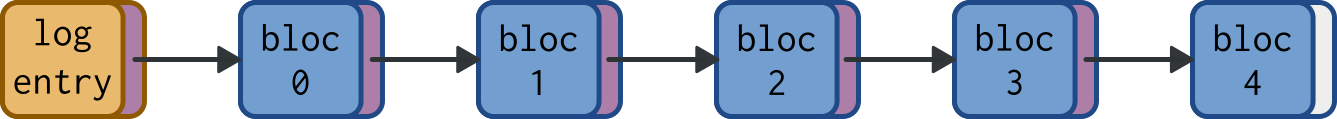
\includegraphics[width=\columnwidth]{imgs/blocs.png}
\caption{Bloc linking representation}
\label{fig:blocs}
\end{figure}

By addressing blocks by their hash blocks the block list is tamper resistance and avoids deduplication. With the convenient side effect of saving disk space and bandwidth on copy operations.

\subsection{View} \label{view}

Systems that allow replicas to diverge must have a way to eventually reconcile two different states. As a CRDT, conflicts at the log level are not possible. However, concurrent operations on the same path can create conflicts at the file system level. The \textit{view} is responsible for providing a conflict resolved version of the log.

The adopted strategy is similar to Bitcoin's \textit{proof-of-work} in the sense that global consensus is not achieved by coordination but by applying deterministic rules to the Merkle DAG. The \textit{view} uses the self-certified properties of the \textit{log} to build a 3-step rulebook for conflict resolution that enables distributed consensus based on \textit{proof-of-authority}.

\begin{enumerate}
\item Select the branch whose contributors have a higher key on the filesystem hierarchy (log entries with incomplete files are ignored until completed). (\textit{proof-of-authority}.
\item If equal, select the branch with more contributors. More nodes agree on the same branch.
\item If equal, select the branch with a higher root hash. Unambiguous, there are no equal hashes.
\end{enumerate}

A consideration when granting higher permissions to an existing key. Related conflicting branches may have been resolved by scoring on higher hierarchy, but with an increase on authority this balance may change. Acknowledging the current ``wining'' branch is required for maintaining state.

\begin{figure}
\centering
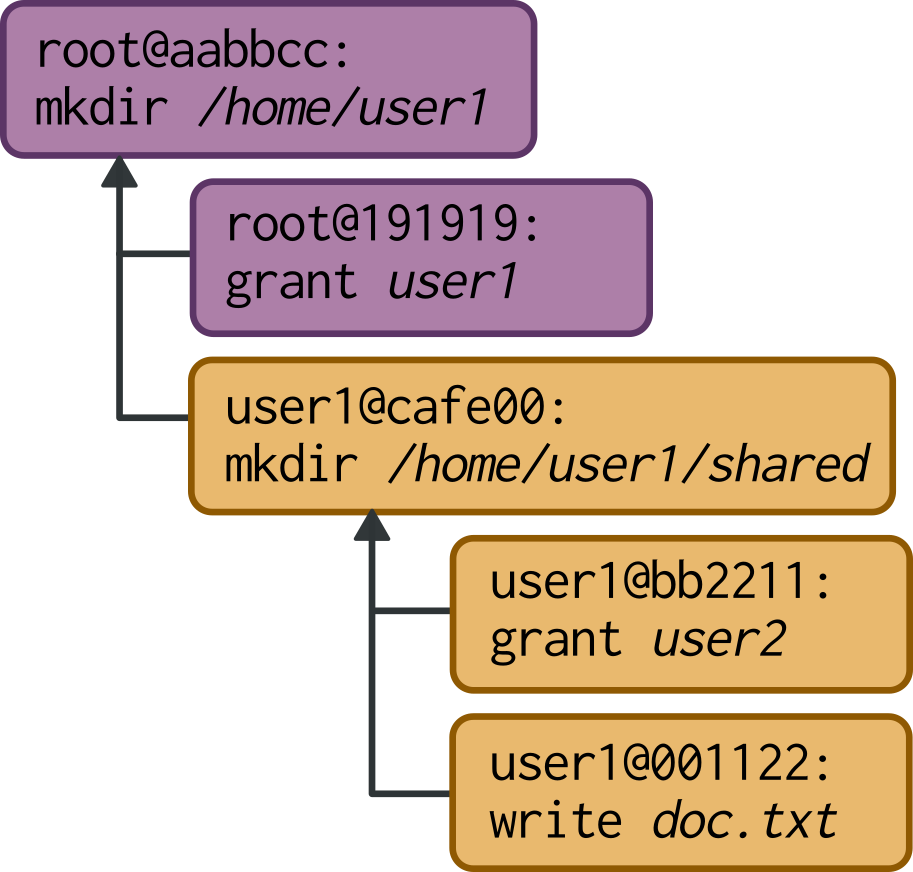
\includegraphics[width=120pt]{imgs/view.png}
\caption{Conflict-free view representation of figure \ref{fig:log} log}
\label{fig:view}
\end{figure}


\subsection{Network} \label{network}

BaseFS uses two different protocols for communicating updates to other nodes and maintain all replicas synchronized:

\begin{itemize}
    \item Gossip protocol - near-real time communication, asynchronous, maintains group membership
    \item Synchronization protocol - anti-entropy protocol for repairing replicated data, compares replicas and reconciles differences
\end{itemize}

Replication is asynchronous, changes are performed locally and then sent to the rest of the network. From the performance perspective this means that the system is fast: the client does not need to spend any additional time waiting for the internals of the system to do their work. The system is also more tolerant to network latency since fluctuations in internal latency do not cause additional waiting.

\subsubsection{Gossip Protocol}\label{gossip-protocol}

A gossip protocol is a style of computer-to-computer communication protocol inspired by the form of gossip seen in social networks. Provides weakly consistent knowledge of group membership to all participants as well as probabilistic broadcast of events to all members. BaseFS uses Serf gossip library, which is based on SWIM, Scalable Weakly-consistent Infection-style Process Group Membership Protocol\cite{SWIM}. Unlike traditional heart-beating protocols, SWIM separates the failure detection and membership update dissemination functionalities of the membership protocol. Processes are monitored through an efficient peer-to-peer periodic randomized probing protocol. Both the expected time to first detection of each process failure, and the expected message load per member, do not vary with group size. Information about membership changes, such as process joins, drop-outs and failures, is propagated via piggybacking on ping messages and acknowledgments. This results in a robust and fast infection style of dissemination. 


\begin{figure*}
\centering

\includegraphics[width=\textwidth]{imgs/payload.png}
\caption{Log entry contained into a Serf custom event payload}
\label{fig:payload}
\end{figure*}

BaseFS uses Serf for a) membership maintenance and b) broadcast of new log entries to the group members. For broadcasting events Serf uses discrete UDP datagrams. UDP is message oriented without ordering, reliable delivery, retransmission nor flow control performed by stream oriented protocols like TCP. It has the limitation of how much information can be sent by a single event. Specifically, Serf allows event payloads as big as 512 bytes. A conscious effort has been made in order to ensure BaseFS log entries do not exceed this capacity. Figure \ref{fig:payload} shows how BaseFS assembles log entries into Serf event payloads, with key optimizations being:

\begin{enumerate}
\item The hash function of choice is SHA-224, the smallest SHA (28B) considered secure\footnote{\url{https://en.wikipedia.org/wiki/SHA-2\#Comparison\_of\_SHA\_functions}}.
\item Use of elliptic curve cryptography with 192 bits key size (equivalent to a 2048b RSA key\footnote{\url{https://tools.ietf.org/html/draft-ietf-msec-mikey-ecc-03}}). Keys of this size produce  48 Bytes signatures.
\item Encoding of the file size value is limited to 6 bytes, restricting the maximum file size to 2 PiB.
\item Even though text protocols are easier to work with, we choose to use a more space-efficient binary representation of the entry fields. When possible, field delimitation is encoded into fields of fixed size. Otherwise, a dedicated offset byte is used, which can delimit up to 255 bytes, allowing file names length similar to other moder filesystems.
\end{enumerate}

To address concerns about how many events will be required for effective configuration management, figure \ref{fig:etc-messages} plots a histogram of the number of messages required for replicating the entire \texttt{/etc} directory of a typical Linux box. Including directories, files and symbolic links. Linux \texttt{/etc} directory contains the system configuration and can be a good representative of an actual large distributed system configuration. Using any of the tested encoding methods, 0.987 of \texttt{/etc} content can be disseminated using at most 10 Serf events per file.

\begin{figure}
\centering
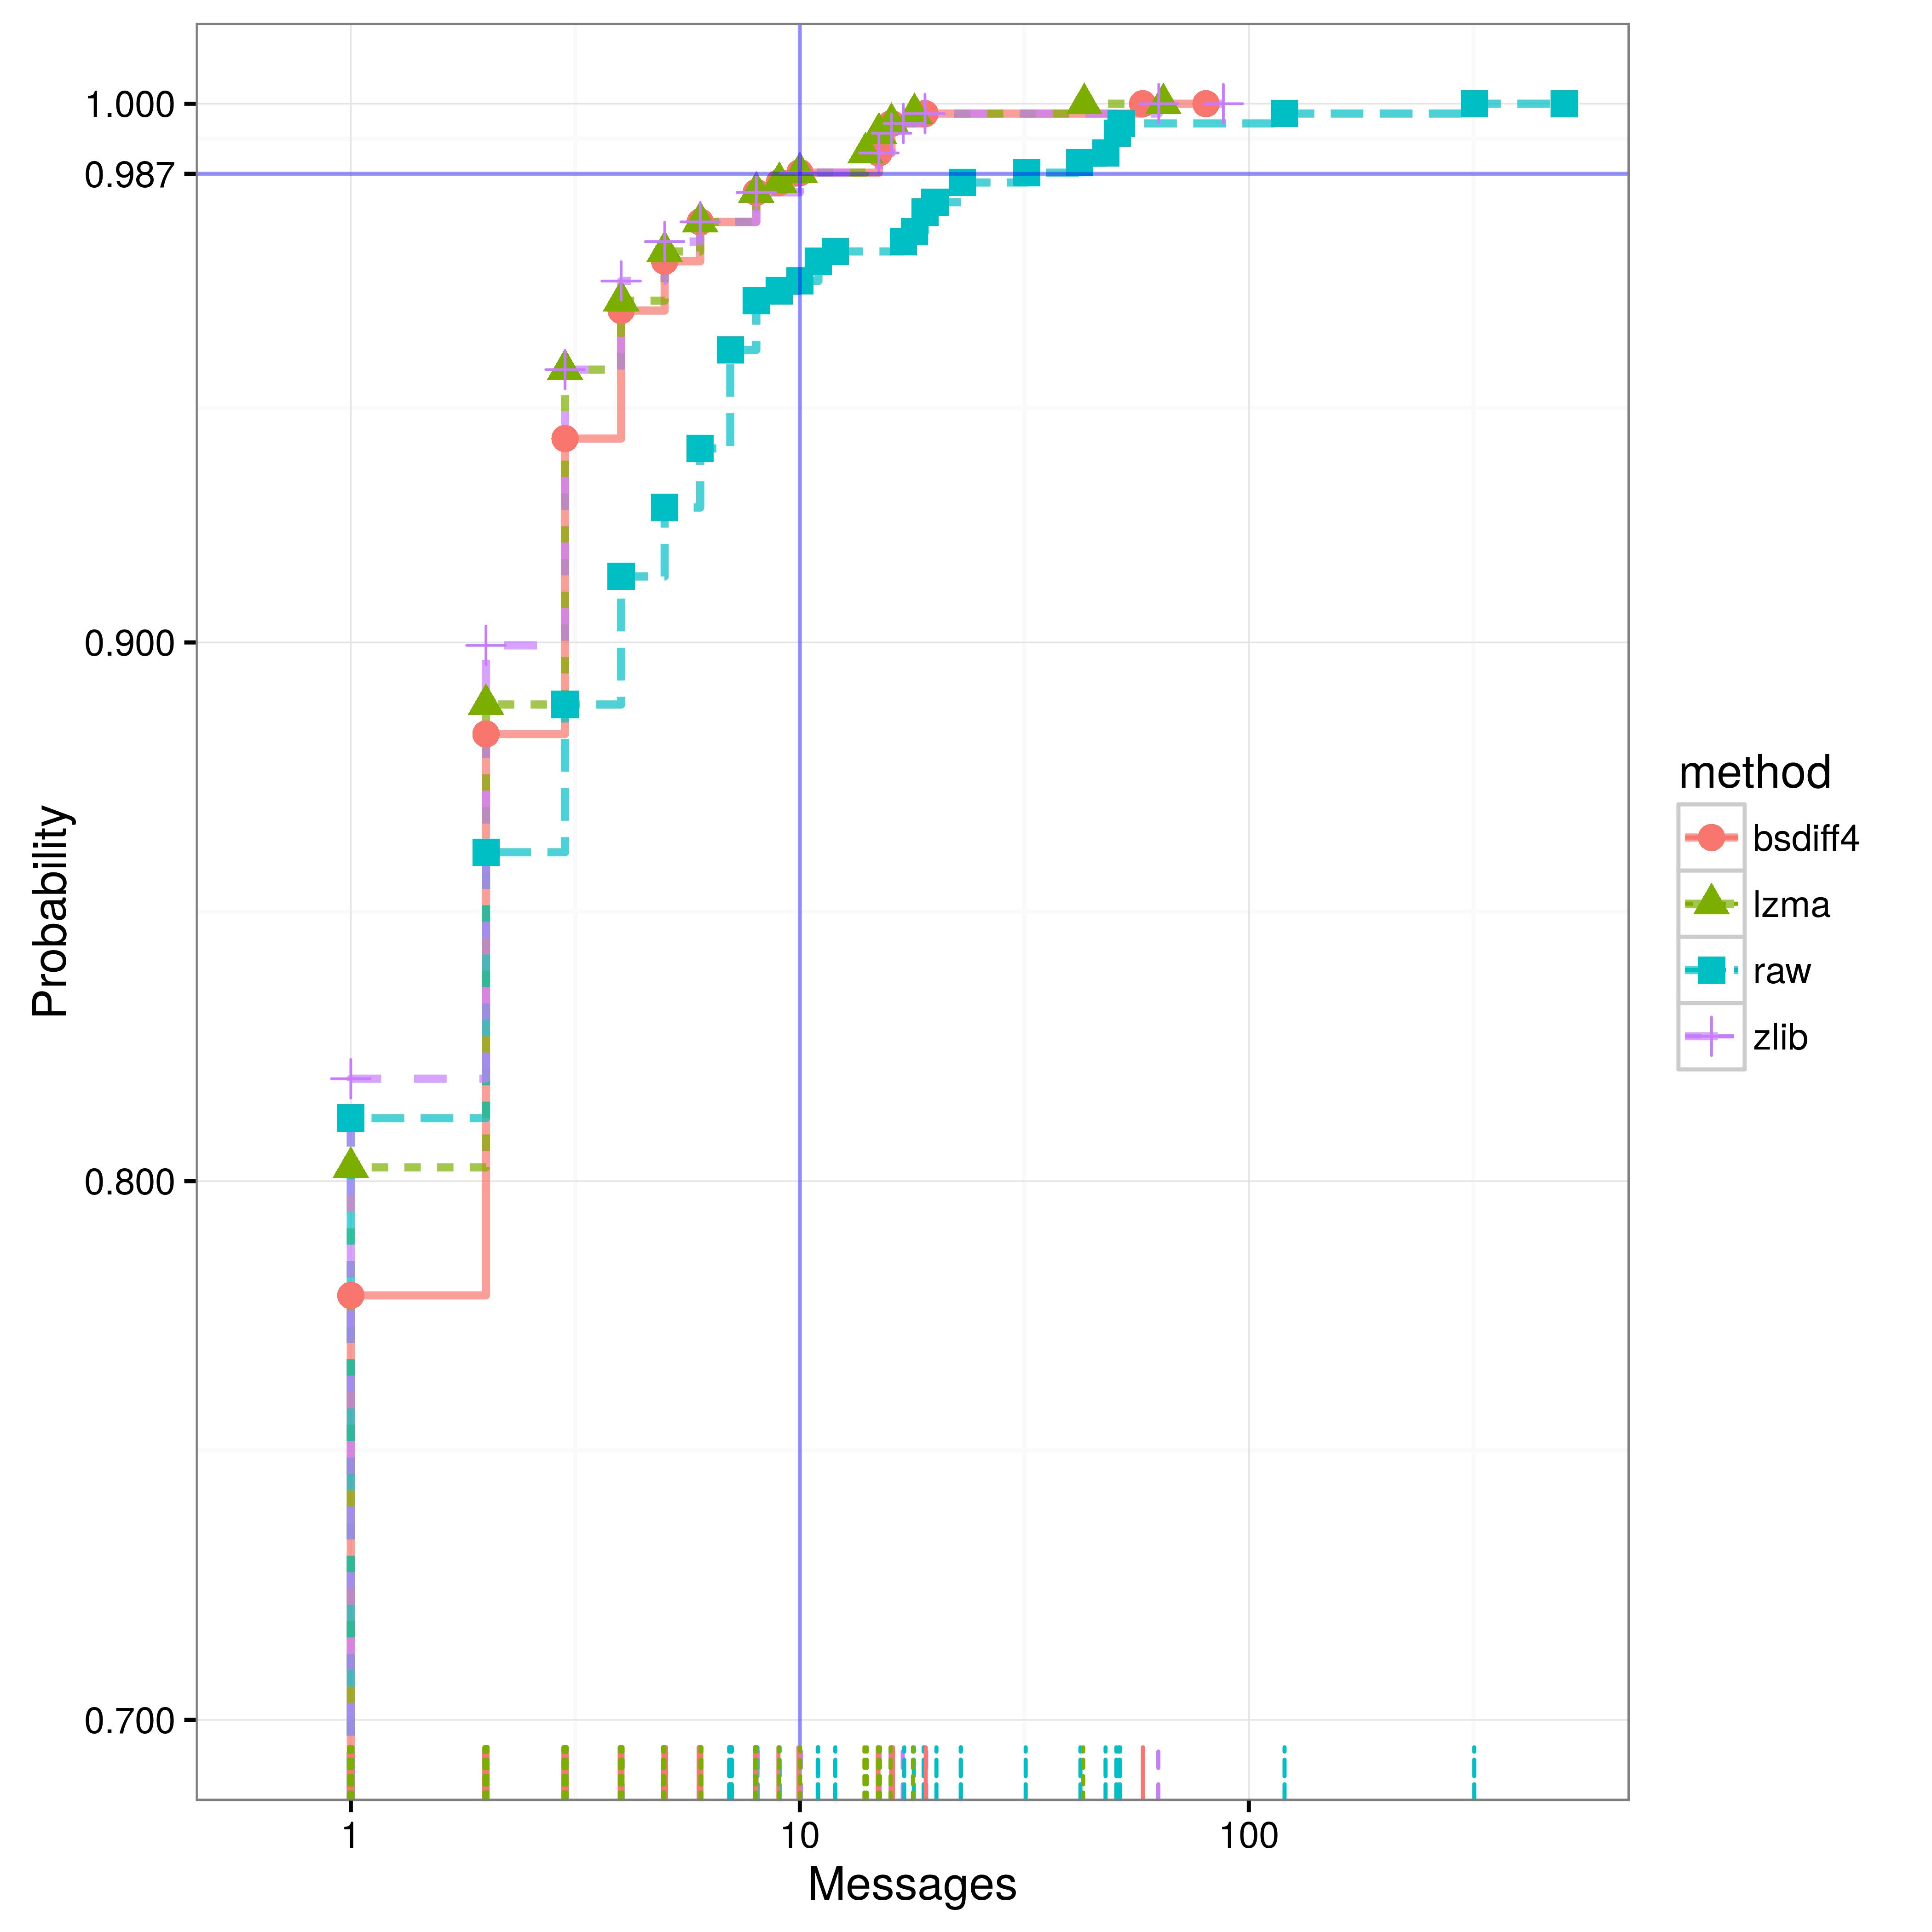
\includegraphics[width=200pt]{imgs/etc_messages.png}
\caption{Cumulative histogram of /etc number of messages}
\label{fig:etc-messages}
\end{figure}

Figure \ref{fig:etc-time} shows the measured time each encoding method takes to process \texttt{/etc} files. Bsdiff4, a tool for building and applying patches to binary files, is perhaps most appropriate method for dynamic configuration. Not only initial patches are comparable in size to other popular compression methods, but the real advantage comes on subsequent file updates. Binary differences between updates are likely to be very small, requiring only one Serf event.

\begin{figure}
\centering
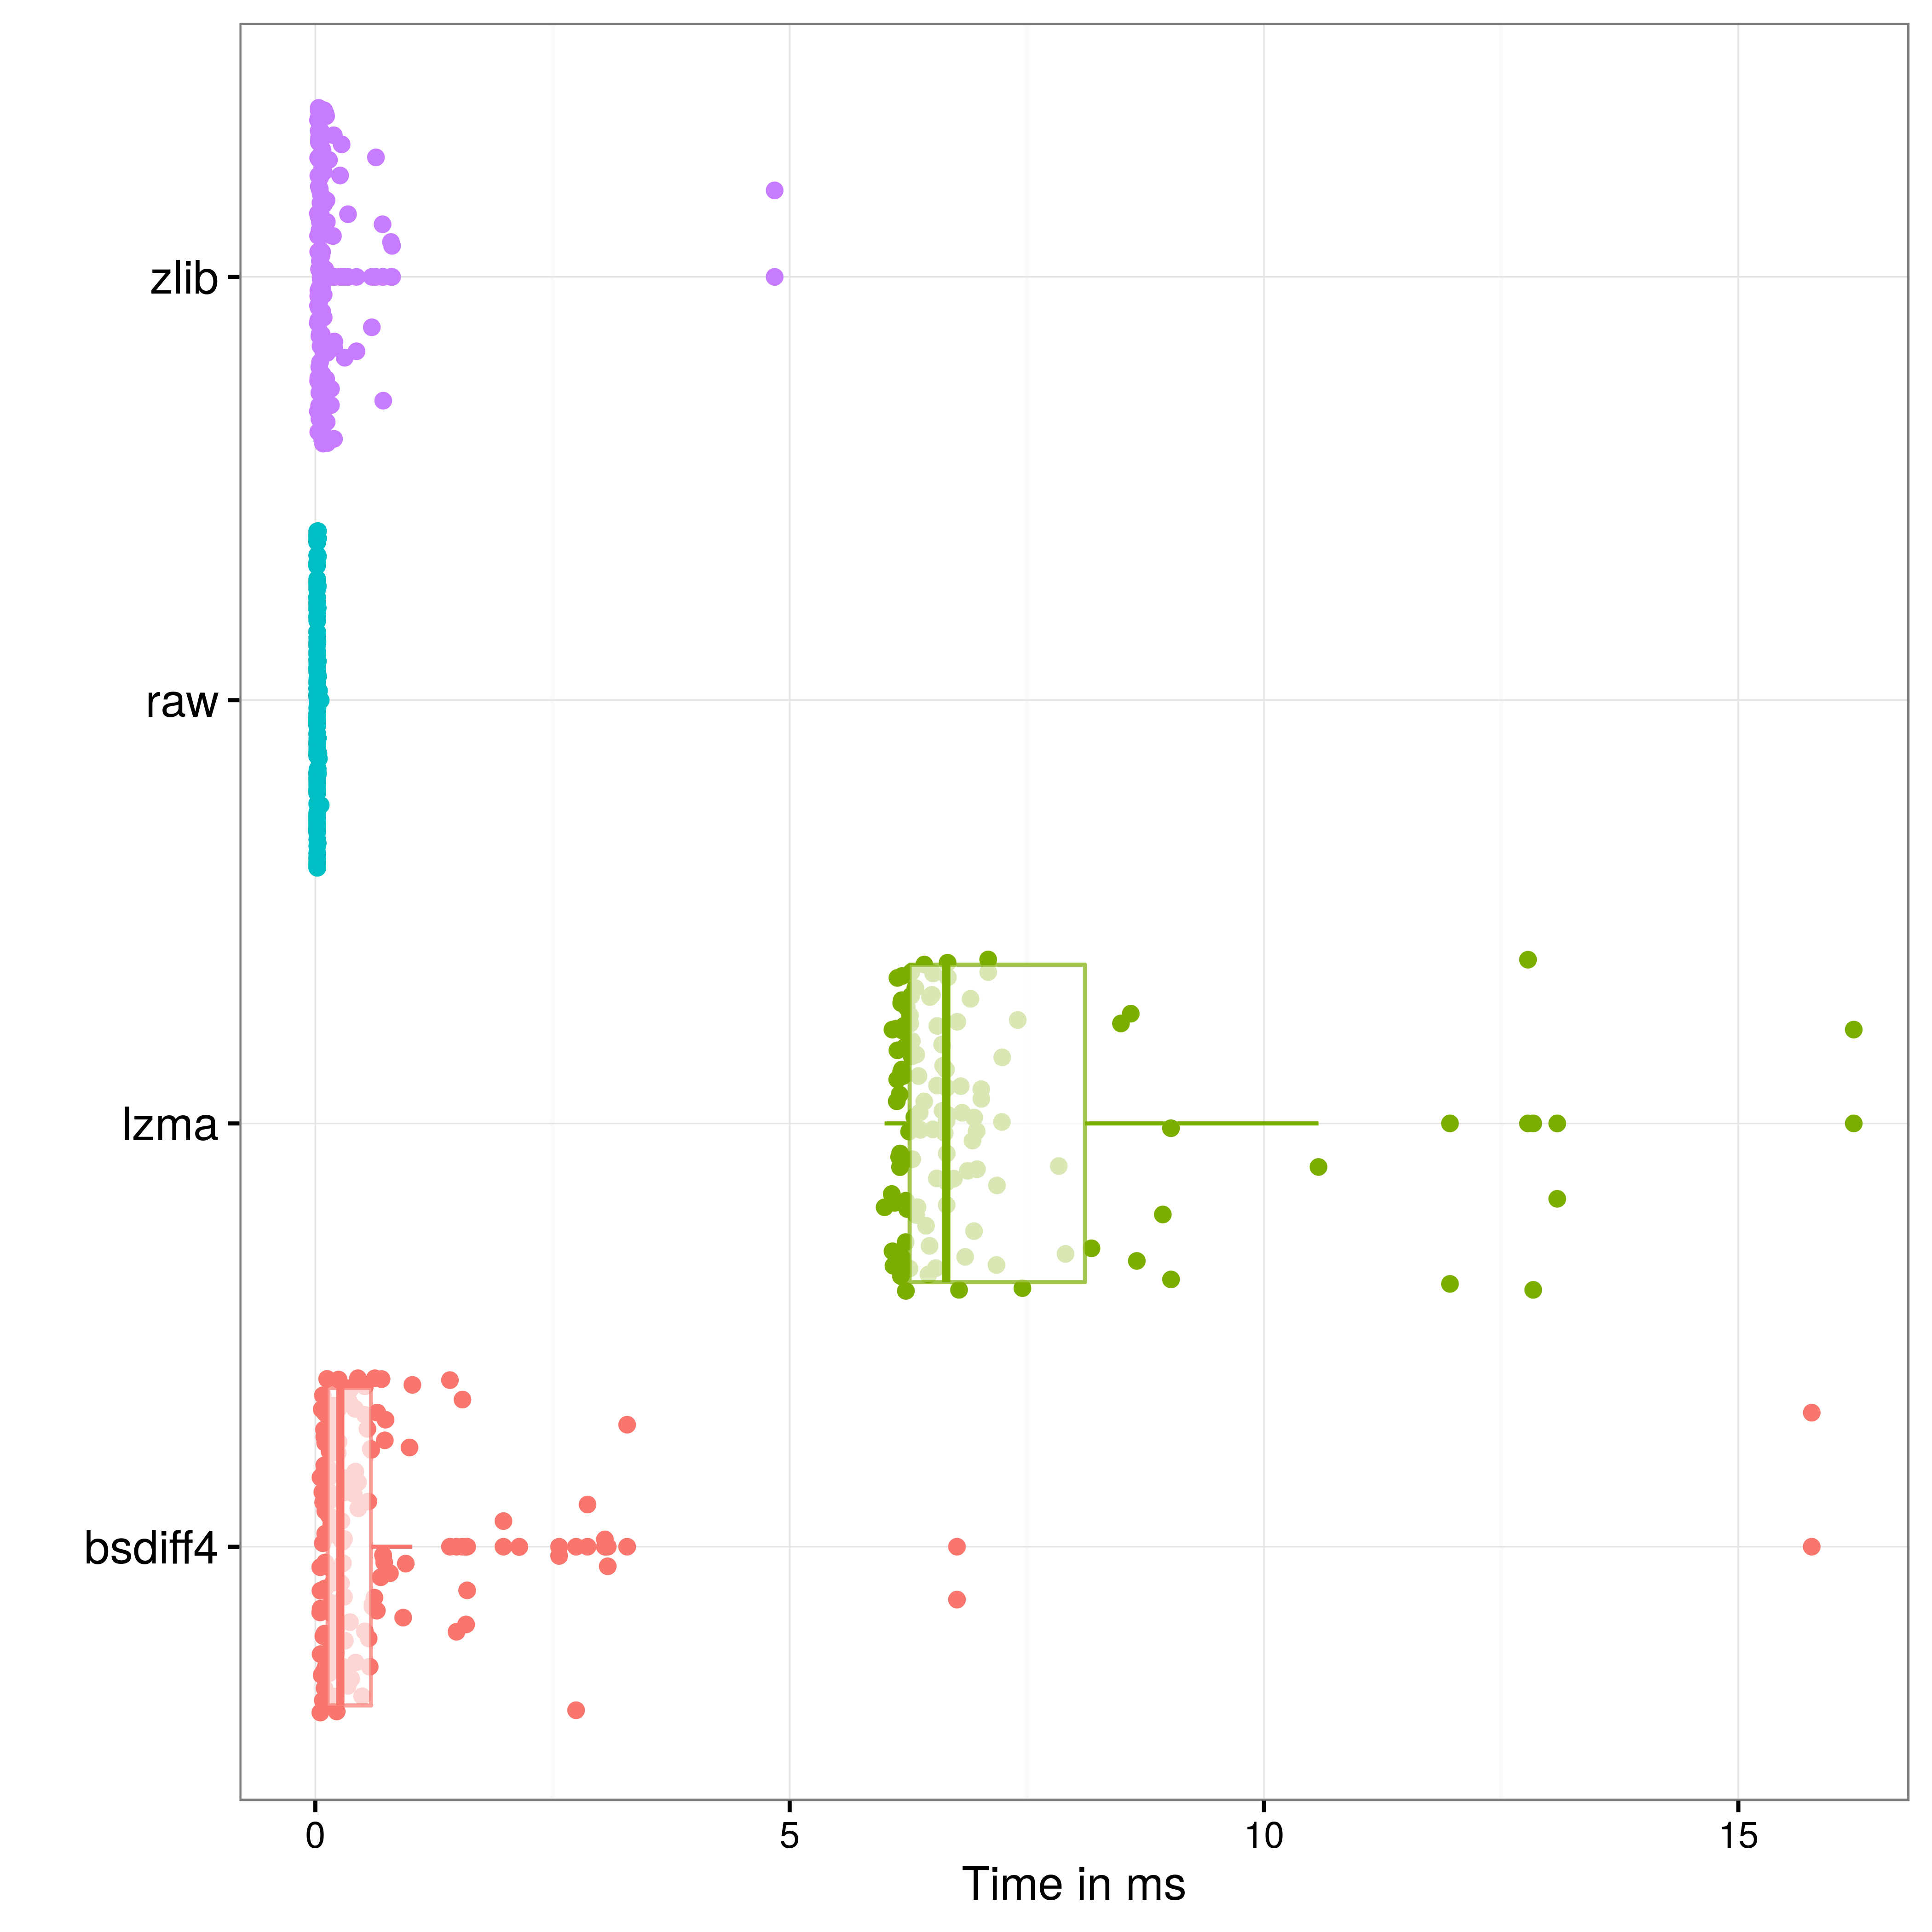
\includegraphics[width=200pt]{imgs/etc_time.png}
\caption{Compression time of /etc files}
\label{fig:etc-time}
\end{figure}



\subsubsection{Synchronization Protocol}

While gossip produces the initial spread of information, a full state synchronization protocol is run infrequently in order to guarantee delivery with probability 1, update nodes after being partitioned and bootstrap nodes joining the system. Additionally, because the number of blocks sent through the gossip layer can be limited by BaseFS configuration, a mechanism to spread remaining blocks is needed. This protocol is different from Serf \textit{full state sync protocol} in two ways. It is not limited to the \textit{nth} most recent events and it is optimized with knowledge of the underlying \textit{log} data structure.

In order to make the information exchange during replica synchronization efficient, the sync protocol uses Merkle trees. Data is hashed at multiple levels of granularity and nodes can quickly find out divergent parts of the data. The Merkle tree is built conforming to the filesystem hierarchy. Each path hash is computed recursively, using the XOR of its sub-paths as well as its own related entries. The root path is the XOR of all log entries. The protocol communication is an iterative process, walking and expanding paths with a mismatching hash. Nodes will detect divergence interchanging log entries and blocks until fully synchronized. 

The synchronization protocol is a text-based streaming protocol. Using new line character as log entry delimiter, spaces as field delimiter and encodes binary content in base64, avoiding delimiters to appear out of place. Its alphabet is:

\begin{itemize}
\item \texttt{HASH} - Filesystem root hash. Identifies the filesystem and avoids inter-filesystem synchronizations. 
\item \texttt{LS} - Path list, includes all path entry hashes, sub-paths hashes and the last-block hash of incomplete files.
\item \texttt{PATH\_REQ} - Path request, indicates a node is missing an entire path and requests all its content to its peer.
\item \texttt{ENTRY\_REQ} - Entry request, used by a node to request a missing entry to its peer.
\item \texttt{BLOCK\_REQ} - idem for blocks
\item \texttt{ENTRIES} - Contains a log entry, can be a response to an \texttt{ENTRY\_REQ} or when a node finds out that its peer is missing some entry.
\item \texttt{BLOCKS} - idem for blocks
\item \texttt{BLOCKS\_REC} - A node announces files in receiving state. In case of divergence the peer can apply this hash to the Merkle tree.
\item \texttt{CLOSE} - Indicates a node is fully synchronize with its peer and communication is terminated.
\item \texttt{EOF} - Signals end of transmission.
\end{itemize}

The pattern of communication is probabilistic, correlated with the amount of time passed since last contact. Every $t$ seconds, a node chooses a peer $i$ with probability $p_i = t_i/\sum_{j=1}^{1,n} t_j$. Synchronization is initiated by sending \texttt{HASH} and \texttt{LS /} requests containing local state. Things continue from there.

To make dissemination faster for files greater than \\ \texttt{MAX\_GOSSIPED\_BLOCKS}, nodes immediately initiate synchronization with a number of peers specified by a configurable \texttt{SEED\_NODES}, defaulting to 4.

Block hashes are not included on the Merkle tree. Doing so will make the synchronization protocol very unstable during periods of gossip dissemination. Whit root hash flapping its value very rapidly. To avoid this effect, as well as preventing nodes to simultaneously retrieve the same blocks from multiple peers, the notion of \textit{block state} is introduce. Files can be in one of the following three states, also represented in figure \ref{fig:blockstate}:

\begin{figure}
\centering
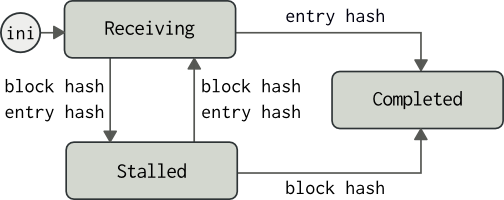
\includegraphics[width=170pt]{imgs/blockstate.png}
\caption{Block state diagram}
\label{fig:blockstate}
\end{figure}


\begin{itemize}
\item Receiving - indicates a node is being receiving blocks. The sync protocol announces the file as being received, so the other replica can account for it when comparing state.
\item Stalled - a file enters this state when no related blocks have been received after some time $t$. Both, the \textit{entry hash} and the \textit{last received block} are added to the Merkle tree.
\item Completed - all file related blocks have been received. The \textit{entry hash} is included to the Merkle tree. In case the previous state was stalled, \textit{last block hash} is removed.
\end{itemize}


\subsection{Filesystem}\label{filesystem}
The filesystem layer provides a well-known API for users and applications to interact with the \textit{view}. The filesystem interface is implemented using FUSE Python bindings\footnote{\url{https://github.com/terencehonles/fusepy}}. FUSE stands for Filesystem in Userspace, and allows developers to build virtual filesystems without having to write kernel modules.

The implementation is very straightforward, almost limited to \textit{View} operations. Only a couple of optimizations are worth mentioning:

\begin{itemize}
 \item The \textit{view layer} does not rebuild automatically when new changes arrive from the network. Instead, the \textit{log seek value} is used to check if the \textit{view} is up-to-date with the \textit{log} on each read. A mismatch indicates new entries have arrived and a rebuild of the \textit{view} is performed before doing the actual read.
 \item File \texttt{writes} are staged until file \texttt{release} is executed. Updates may require multiple \texttt{write} operations, BaseFS waits until file \texttt{release} to actually write changes to the \texttt{view}. Benefits being a) generate a single Bsdiff4 patch and b) summarizes all related \texttt{writes} into a single log entry.
\end{itemize}


\subsubsection{Watchers}\label{watchers}
The naive approach for applications to react to changes is periodic reading (pulling) the state they are interested in. Modern Linux kernels provide support for filesystem notifications via the \textit{inotify} subsystem. Unfortunately FUSE has no support for triggering \textit{inotify} events. BaseFS provides support for executing scripts in response to new log entries in the form of event handlers.

Event handlers are registered at mount time and are invoked in the context of a shell. Can be any executable, including piped executables (such as \texttt{awk '{print \$2}' | grep foo}). Event handlers are executed anytime a new log entry is stored. Context for the scripts is given by environment variables such as \texttt{BASEFS\_EVENT\_TYPE} and \texttt{BASEFS\_EVENT\_PATH}.

\subsection{Modules Overview}\label{modules}

Figure \ref{fig:modules} shows the main BaseFS modules and their interactions. BaseFS makes extensive use of concurrency including processes, threads and an event loop. The FUSE interface runs on the main Python thread, as required by its implementation. The Serf agent runs on a separated Python process. Communication with Serf agent is done using Serf's RPC protocol. We spawn an additional thread for the event loop. Implemented with \textit{asyncio}, the event loop handles all the remaining network communication in a non-blocking fashion. Including the synchronization protocol, receiving of gossip events and commands sent by BaseFS CLI utility. The event loop thread shares memory with the main FUSE thread, and only a single instance of the \textit{view} has to be maintained, saving substantial memory and computation time.

The modular design allows for easy module replacement. For example, the filesystem module providing a convenient filesystem API to the \textit{view} can be replaced, or complemented, by other interfaces, like HTTP REST.

\begin{figure}
\centering
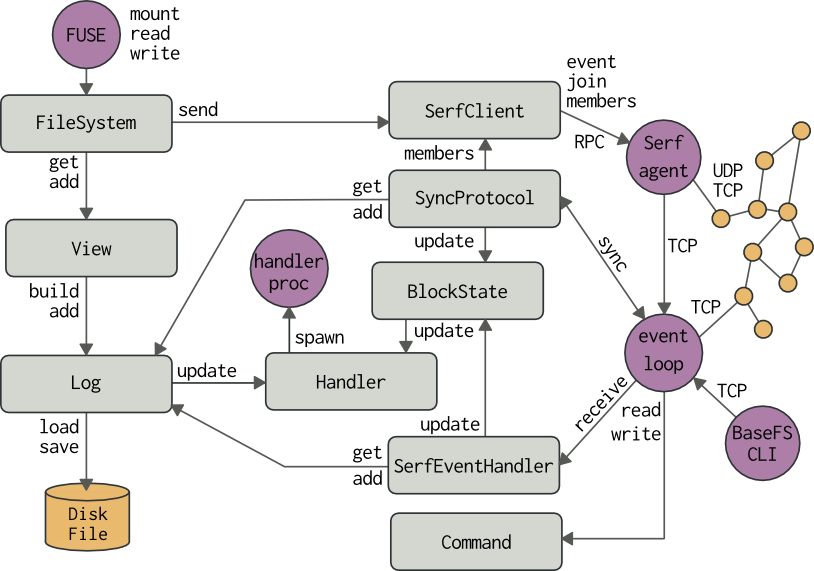
\includegraphics[width=\columnwidth]{imgs/modules.png}
\caption{BaseFS modules}
\label{fig:modules}
\end{figure}

\subsubsection{CLI Commands}
The filesystem API is limited to data operations. For administration and management purposes BaseFS provides a command line tool that talks to BaseFS daemon via a simple text-based TCP protocol. Some of the commands are:

\begin{itemize}
 \item \texttt{mount}	Mount an existing filesystem
 \item \texttt{run}	Run node without mounting
 \item \texttt{bootstrap}	Create a new self-contained filesystem
 \item \texttt{genkey}	Generate a new EC private key
 \item \texttt{keys}	List keys and their directories
 \item \texttt{grant}	Grant key write permission
 \item \texttt{revoke}	Revoke key write permission
 \item \texttt{list}	List all available logs
 \item \texttt{show}	Show a log file using a tree representation
 \item \texttt{revert}	Revert object to previous state
 \item \texttt{blocks}	Show block state of incomplete files
 \item \texttt{members}	List group members
 \item \texttt{get}		Get log from peer address
 \item \texttt{resources}	Monitor resource consumption in real-time
\end{itemize}


\section{Evaluation} \label{evaluation}

In this section an evaluation of the BaseFS network properties and IO performance is presented. For the validation of the Merkle DAG conflict resolution and permissions the reader can refere to the unit and functional tests shipped with BaseFS source code\footnote{\url{https://github.com/glic3rinu/basefs/}}.

All test scenarios have been fully automated for easily reproducibility. We have developed our own test suite. The test suite has support for virtual environments based on Docker containers, as well as support for deploying and running experiments on Community-Lab testbed\cite{selimi2014cloud}. Docker builds on top of the Linux kernel resource isolation features to provide operating-system-level virtualization. Community-Lab is a Community Netwotk Testbed by the CONFINE project that provides a global facility for experimentation with network technologies and services for community networks. 

The machine used for running virtual experiments is an Intel(R) Core(TM) i7-4500U CPU @ 1.80GHz, with 4 cores and 7GB of memory.


\subsection{Network Evaluation}
The network evaluation is separated into two phases that determine a) how constrained network characteristics affect BaseFS convergence time and b) how BaseFS behaves in a real Community Network environment. 

Docker containers use virtual Ethernet devices connected to a virtual bridge. All nodes are at one layer 2 hop between each other. TC (Linux Traffic Control) is used for configuring the kernel network scheduler and shape the traffic characteristics of the virtual network. Each experiment is performed on a group of 30 nodes. For each experiment a new BaseFS log is bootstrapped. Nodes get and mount this freshly created BaseFS filesystem. Group members are given a few seconds to find each other. We simulate configuration updates by copying a set of pre-created files into one of the nodes BaseFS mounted partition. Then we measure the time it takes for the configuration file to propagate to the rest of the group. We monitor the number of converged nodes in real time, so the experiment can advance as soon as all nodes have received the updates. We define a maximum waiting time of 100 minutes between file copies, with an additional maximum of 150 minutes at the end of each experiment.


\subsubsection{Prelude: Parametrization}

Before performing the evaluation we will choose the value of some important BaseFS parameters and environment conditions. In particular we want to establish a sane limit on the \textit{number of blocks sent by the gossip layer}, a good value for the \textit{full state synchronization execution frequency} and which is the \textit{maximum number of Docker containers} we can run without significant CPU contention.


\paragraph{Maximum gossiped blocks}

Gossip capacity is limited by available bandwidth and CPU cycles for generating and processing messages. Under high update load, a gossip protocol may not be able to send all updates required to reconcile differences between peers. Updates would take arbitrary time to propagate as the gossip channel gets backed up. \cite{van2008efficient}

Sending large files through a gossip channel is very inefficient. For establishing a good limit on the number of blocks sent by the gossip layer we have generated a collection of files that produce from 1 to 256 gossip messages. The measured time required for a group of 30 nodes to converge is shown on figure \ref{fig:gossip}. Notice that the sync protocol has been disabled for this test.

\begin{figure}
\centering
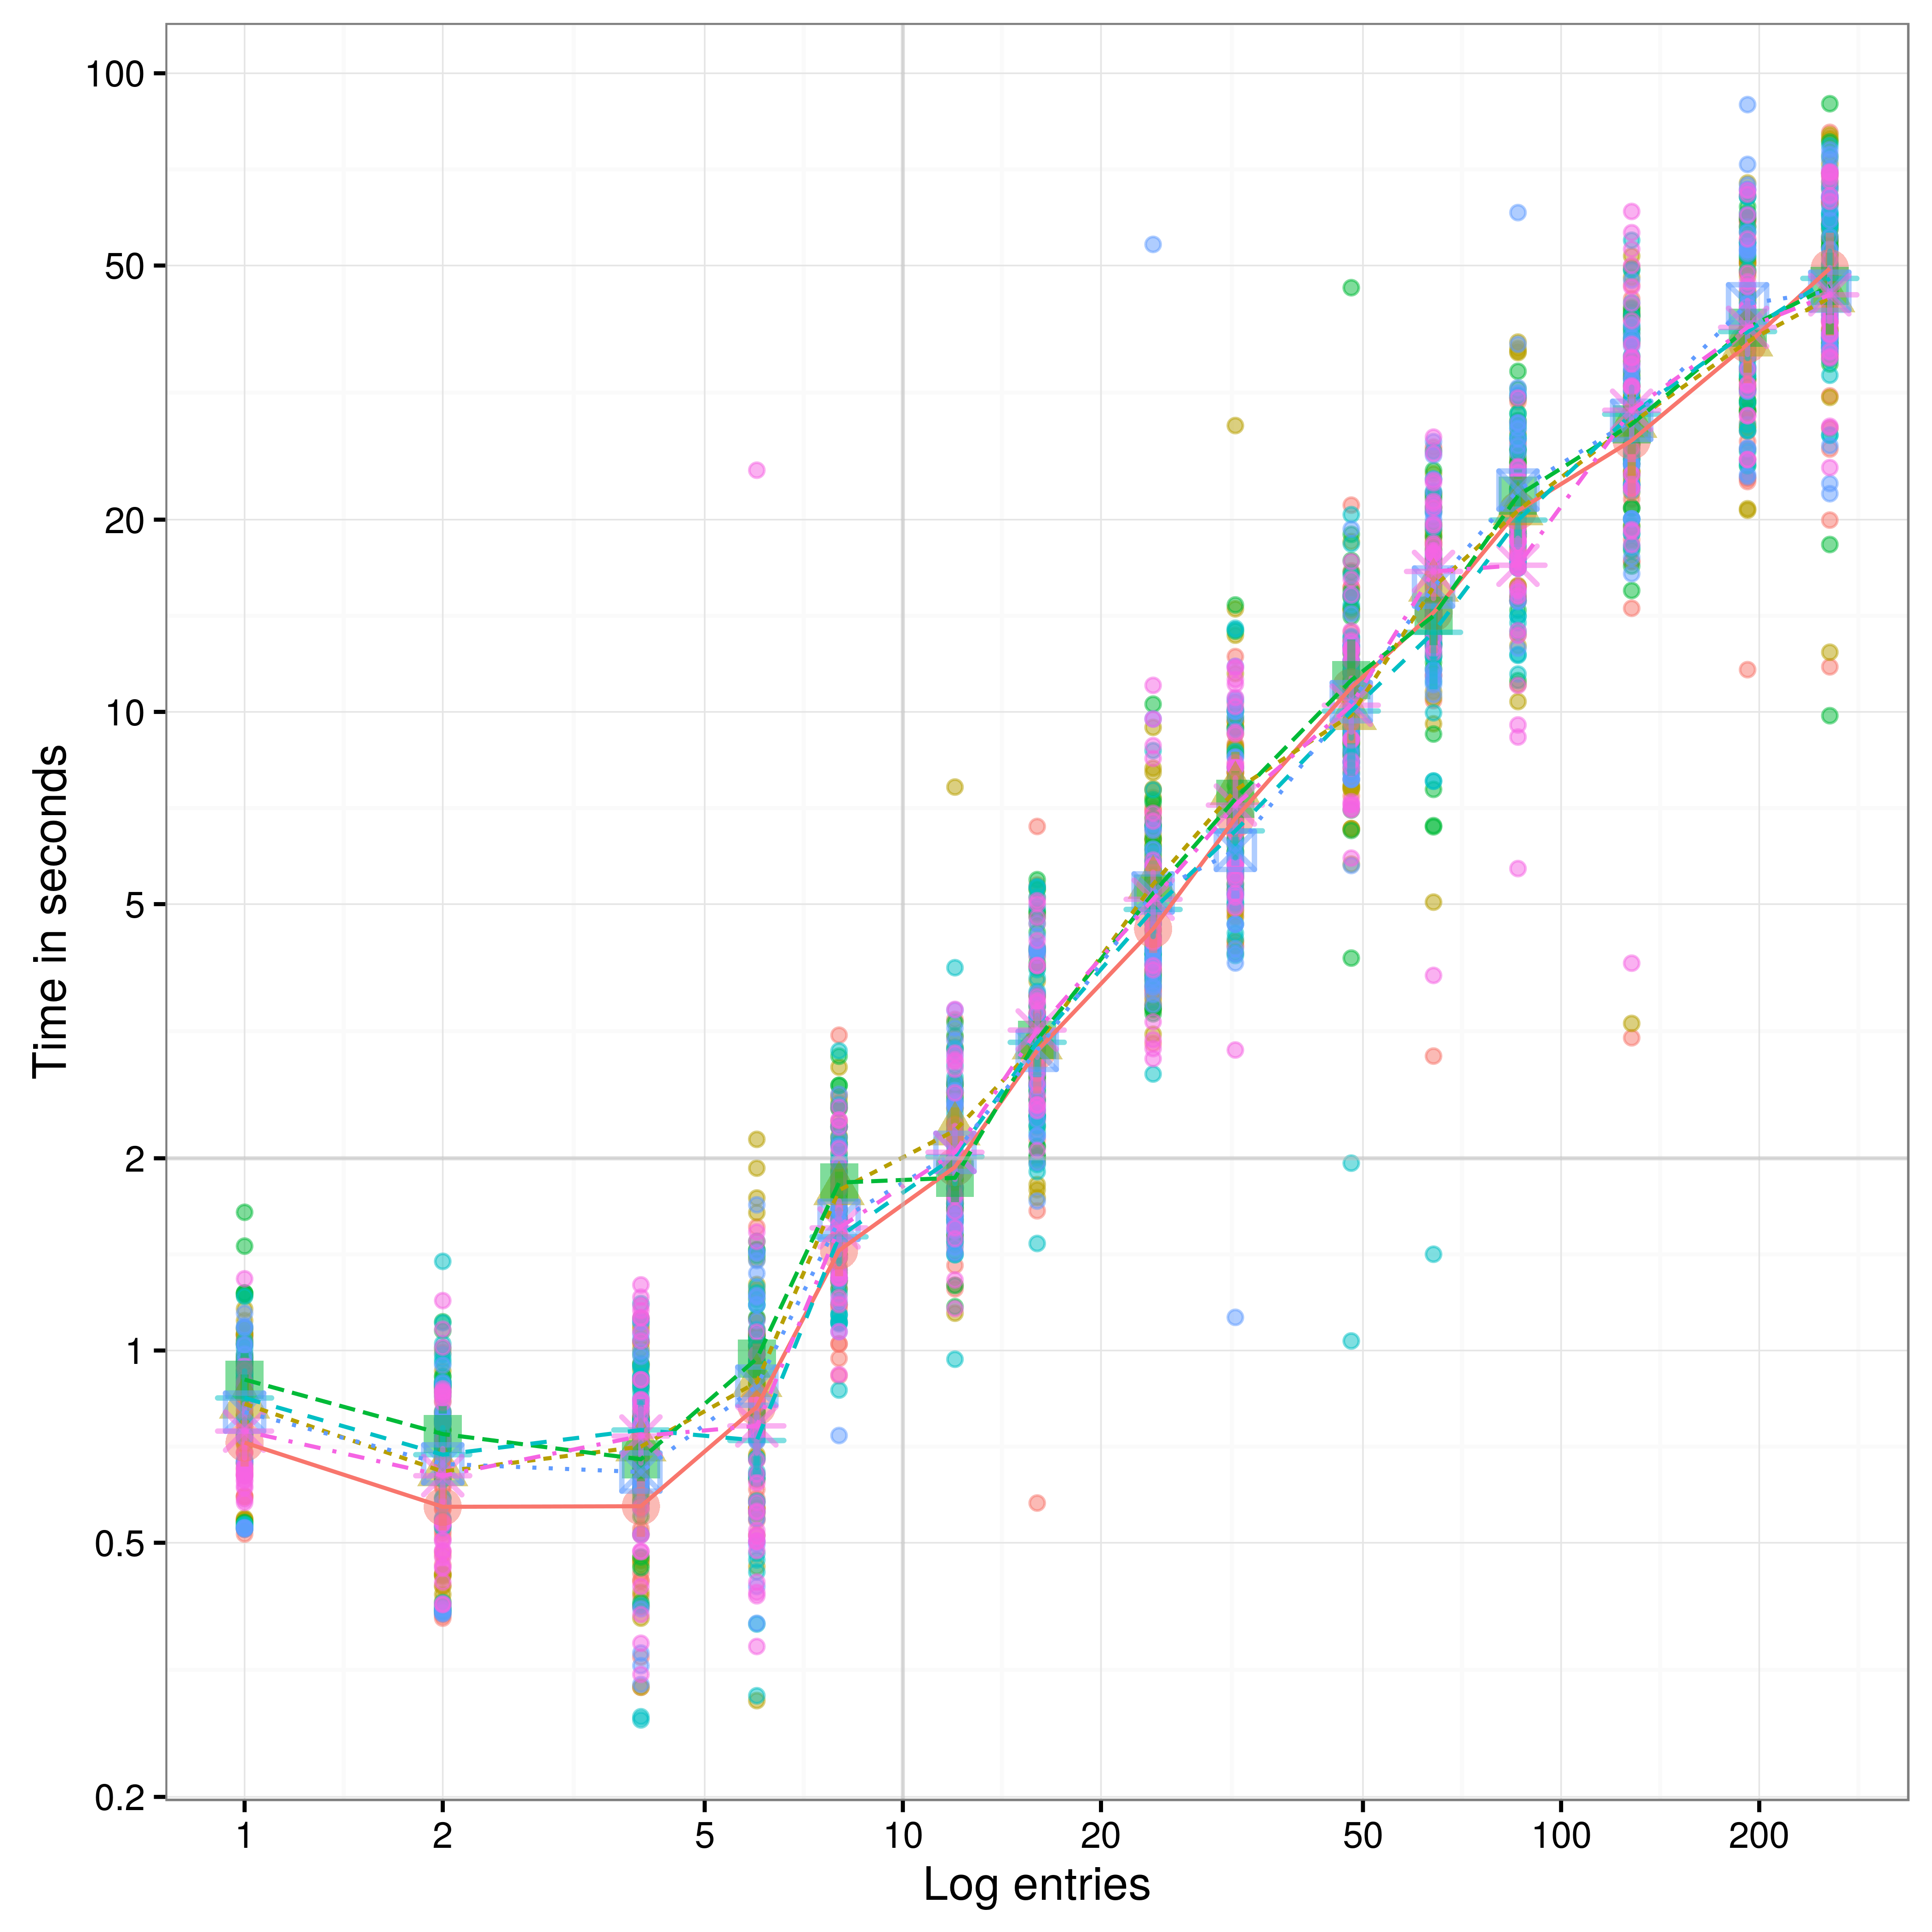
\includegraphics[width=200pt]{imgs/gossip.png}
\caption{Gossip convergence with variable number of gossip messages}
\label{fig:gossip}
\end{figure}

The gossiped blocks limit for our experiments is set to 10. Being a good compromise between mean convergence time (2 seconds, figure \ref{fig:gossip}) while including a large amount of potential files that can be sent (0.987\% of \textit{/etc} content, figure   \ref{fig:etc-messages}).


\paragraph{Synchronization interval}

The frequency at which the synchronization protocol is executed determines the convergence time of the group and how much network traffic is required. Measures with different intervals have been done and summarized in figure \ref{fig:sync}.

\begin{figure}
\centering
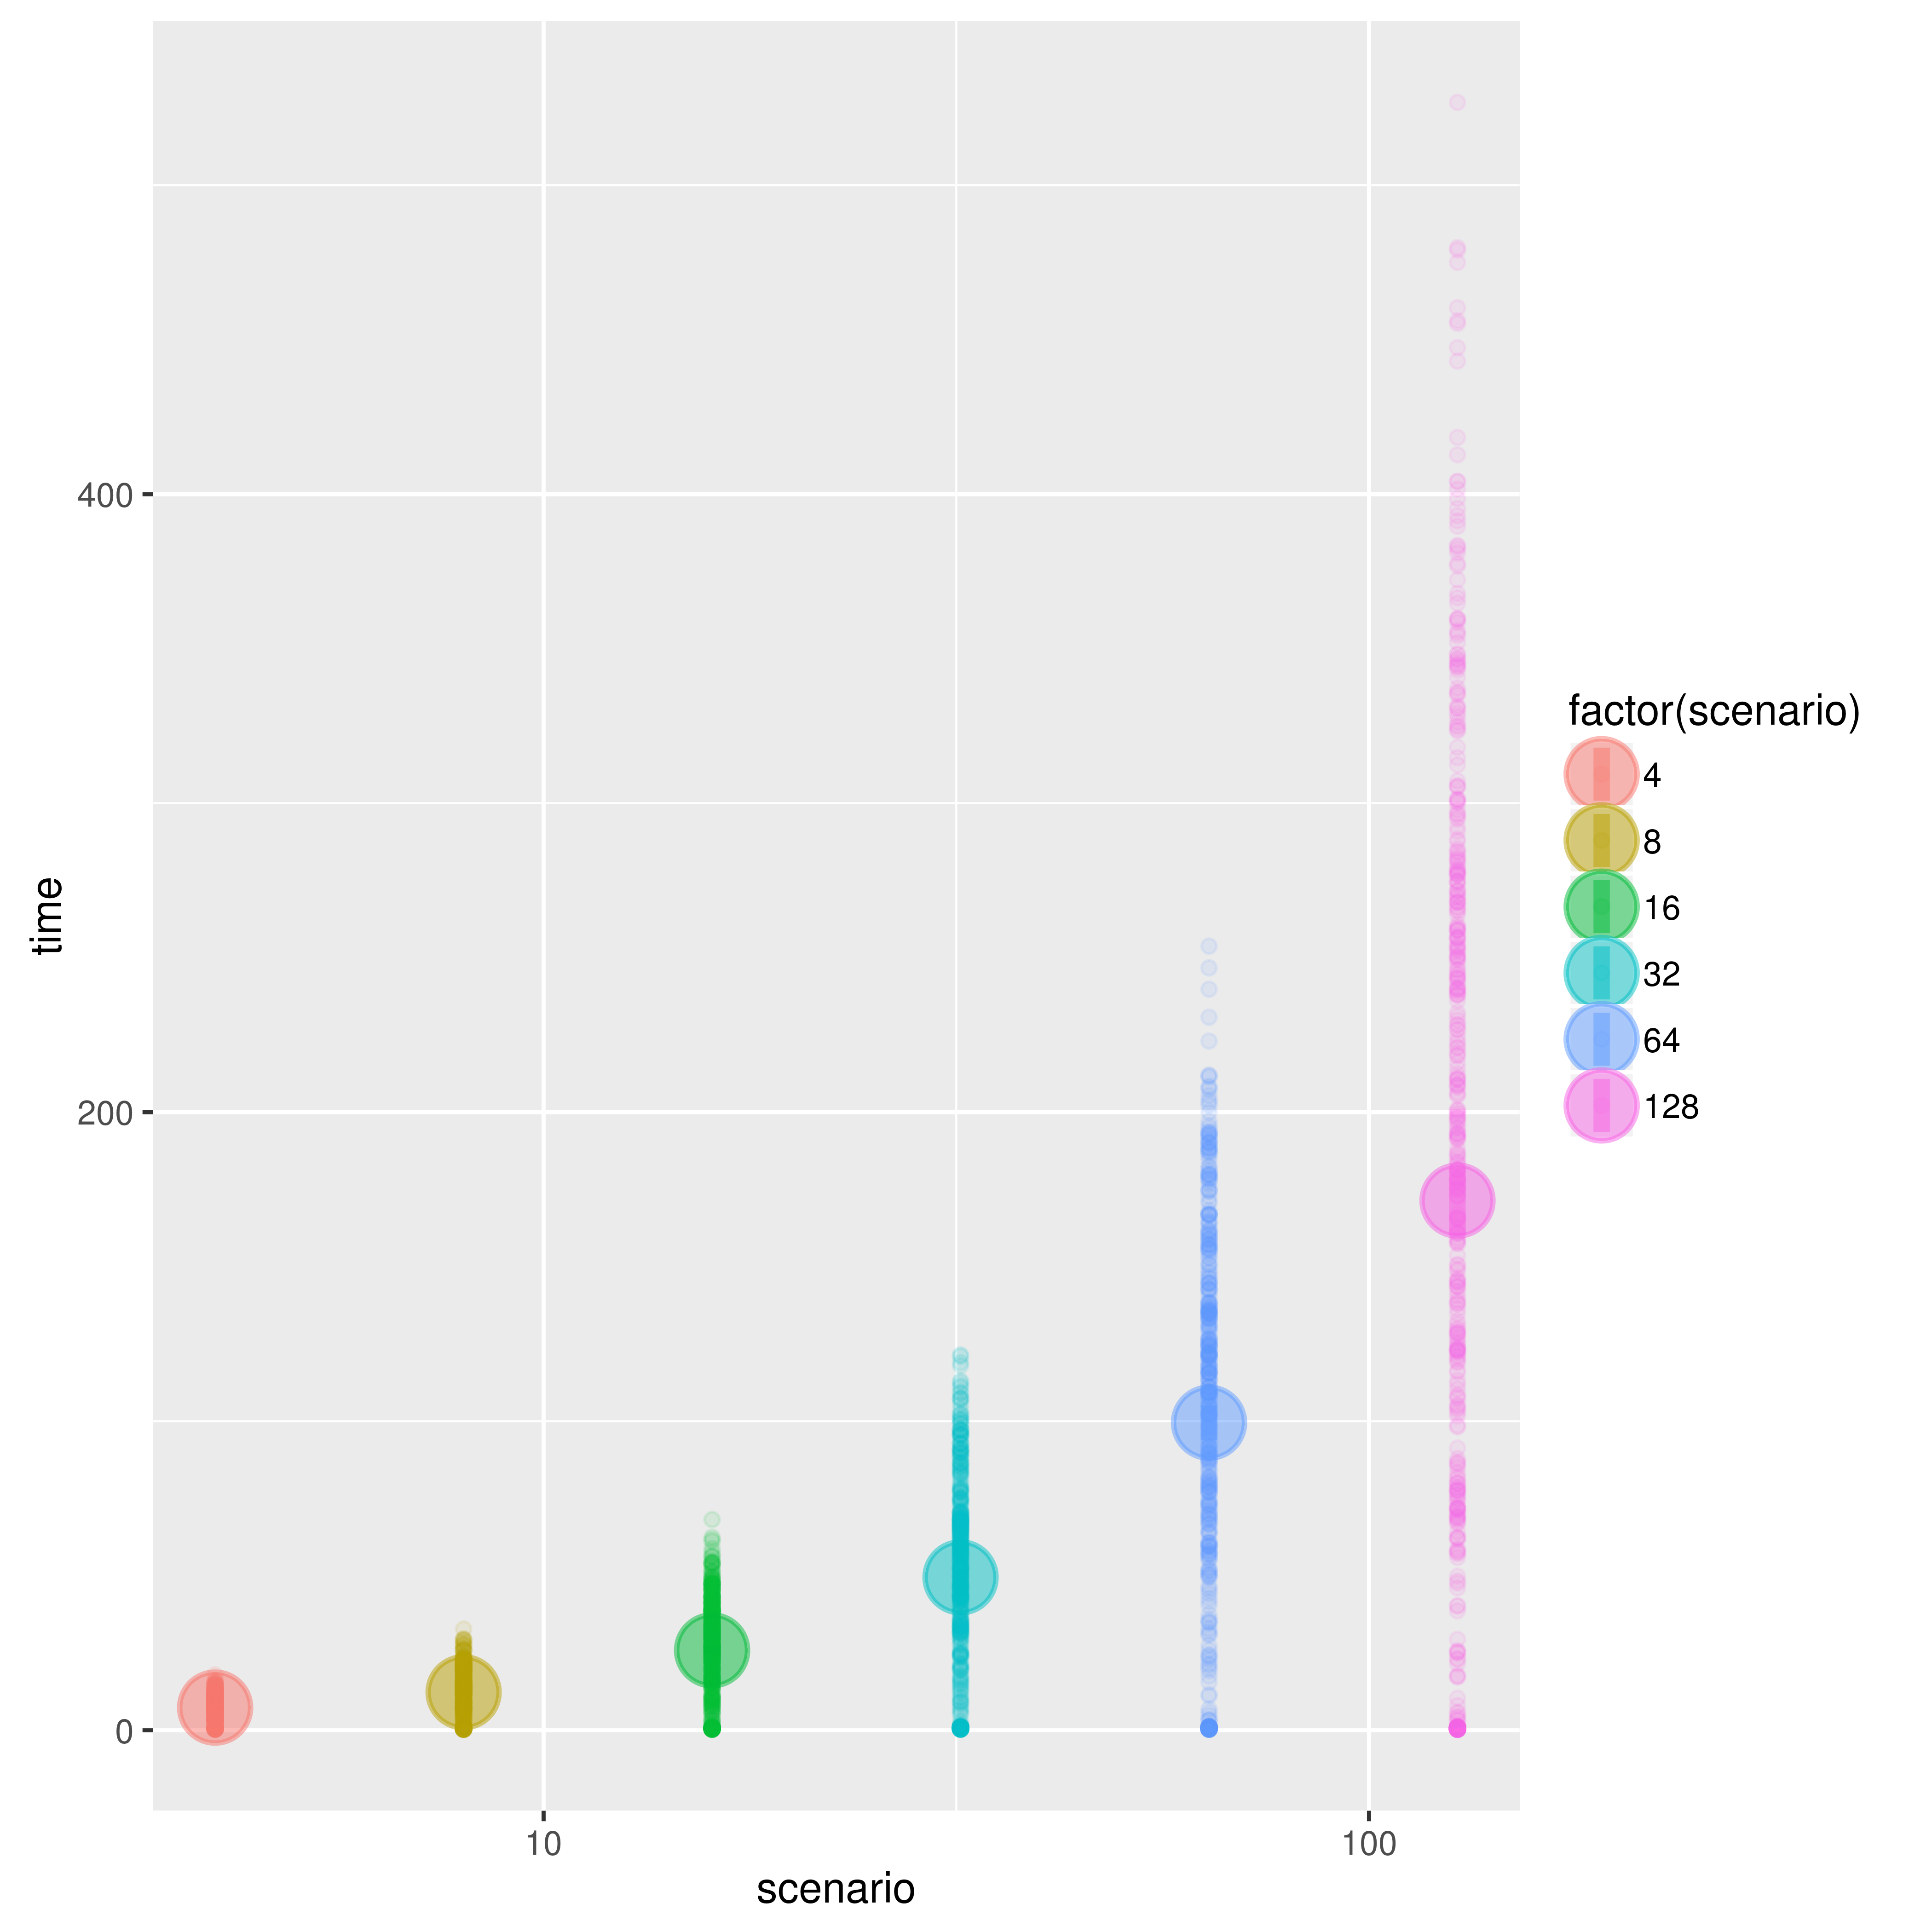
\includegraphics[width=\columnwidth]{imgs/sync.png}
\caption{Full Sync protocol convergence with variable execution interval}
\label{fig:sync}
\end{figure}

We found \textbf{20 seconds} to be a decent default for the synchronization protocol. More than 20 seconds do not significatively increase the amount of traffic, measured at around 2.5Kbps, while giving a reasonable mean convergence time of 30 seconds, with an approximate worst case of 100 seconds. In any case, only 0.013\% of \texttt{/etc} content are files big enough (>10 blocks) to fully depend on the synchronization protocol for their replication.


\paragraph{Number of Docker containers}

CPU contention is what effectively limits the maximum number of BaseFS nodes that can be emulated on a single machine without compromising measurements. Figure \ref{fig:scalability} shows the \textit{1 minute load average}\footnote{Number of jobs in the run queue or waiting for disk IO averaged over 1 minute} of the system while performing 20 writes (separated by 3 seconds) on various group sizes. Writes are crafted to generate predetermined amount of gossip packets, simulating the workload of upcoming experiments. The system is overload starting from 50 containers and hitting swap at 300. We finally choose a conservative group size of 30 nodes, since the computer is also used by other tasks besides running experiments.


\begin{figure}
\centering
\includegraphics[width=\columnwidth]{imgs/scalability.png}
\caption{BaseFS Docker scalability}
\label{fig:scalability}
\end{figure}


% On a 4 core machine, the amount of load average below 4 is interpreted as idle and the amount of load beyond 4 is considered overload. A cluster size below 50 nodes do not has significative CPU contention. But, since the computer is used by other tasks besides running experiments, a more conservative size of \textbf{30 nodes} has been finally chosen for the experiments. As an interesting fact, the convergence time spikes at 300 nodes due to exhaustion of the system's main memory, forcing processes to migrate into swap memory (swapping). Each BaseFS process consumes around 2400KB of resident memory, and the total system memory is 7688200K.

This scalability test has uncovered two caveats of our virtual environment. First, the default value for the neighbor table garbage collector thresholds in the system were set too low, producing overflows on the ARP table\footnote{https://github.com/hashicorp/serf/issues/263}. Another problem of tearing up and down hundreds of Docker containers is running out of IPv4 addresses because of a Docker bug\footnote{https://github.com/docker/docker/issues/14788}. The adopted solution is restarting Docker before each experiment. 


\subsubsection{Delay Effects}

Figure \ref{fig:basefs-delay} shows the measured convergence time of operations with different number of log entries and delay distributions on a virtual group of 30 nodes. The delay distributions are created using \textit{TC netem discipline} (e.g. \texttt{netem delay 100ms 20ms distribution normal}). The standard deviation is kept proportional on each case, always 20\% of the mean.

\begin{figure}
\centering
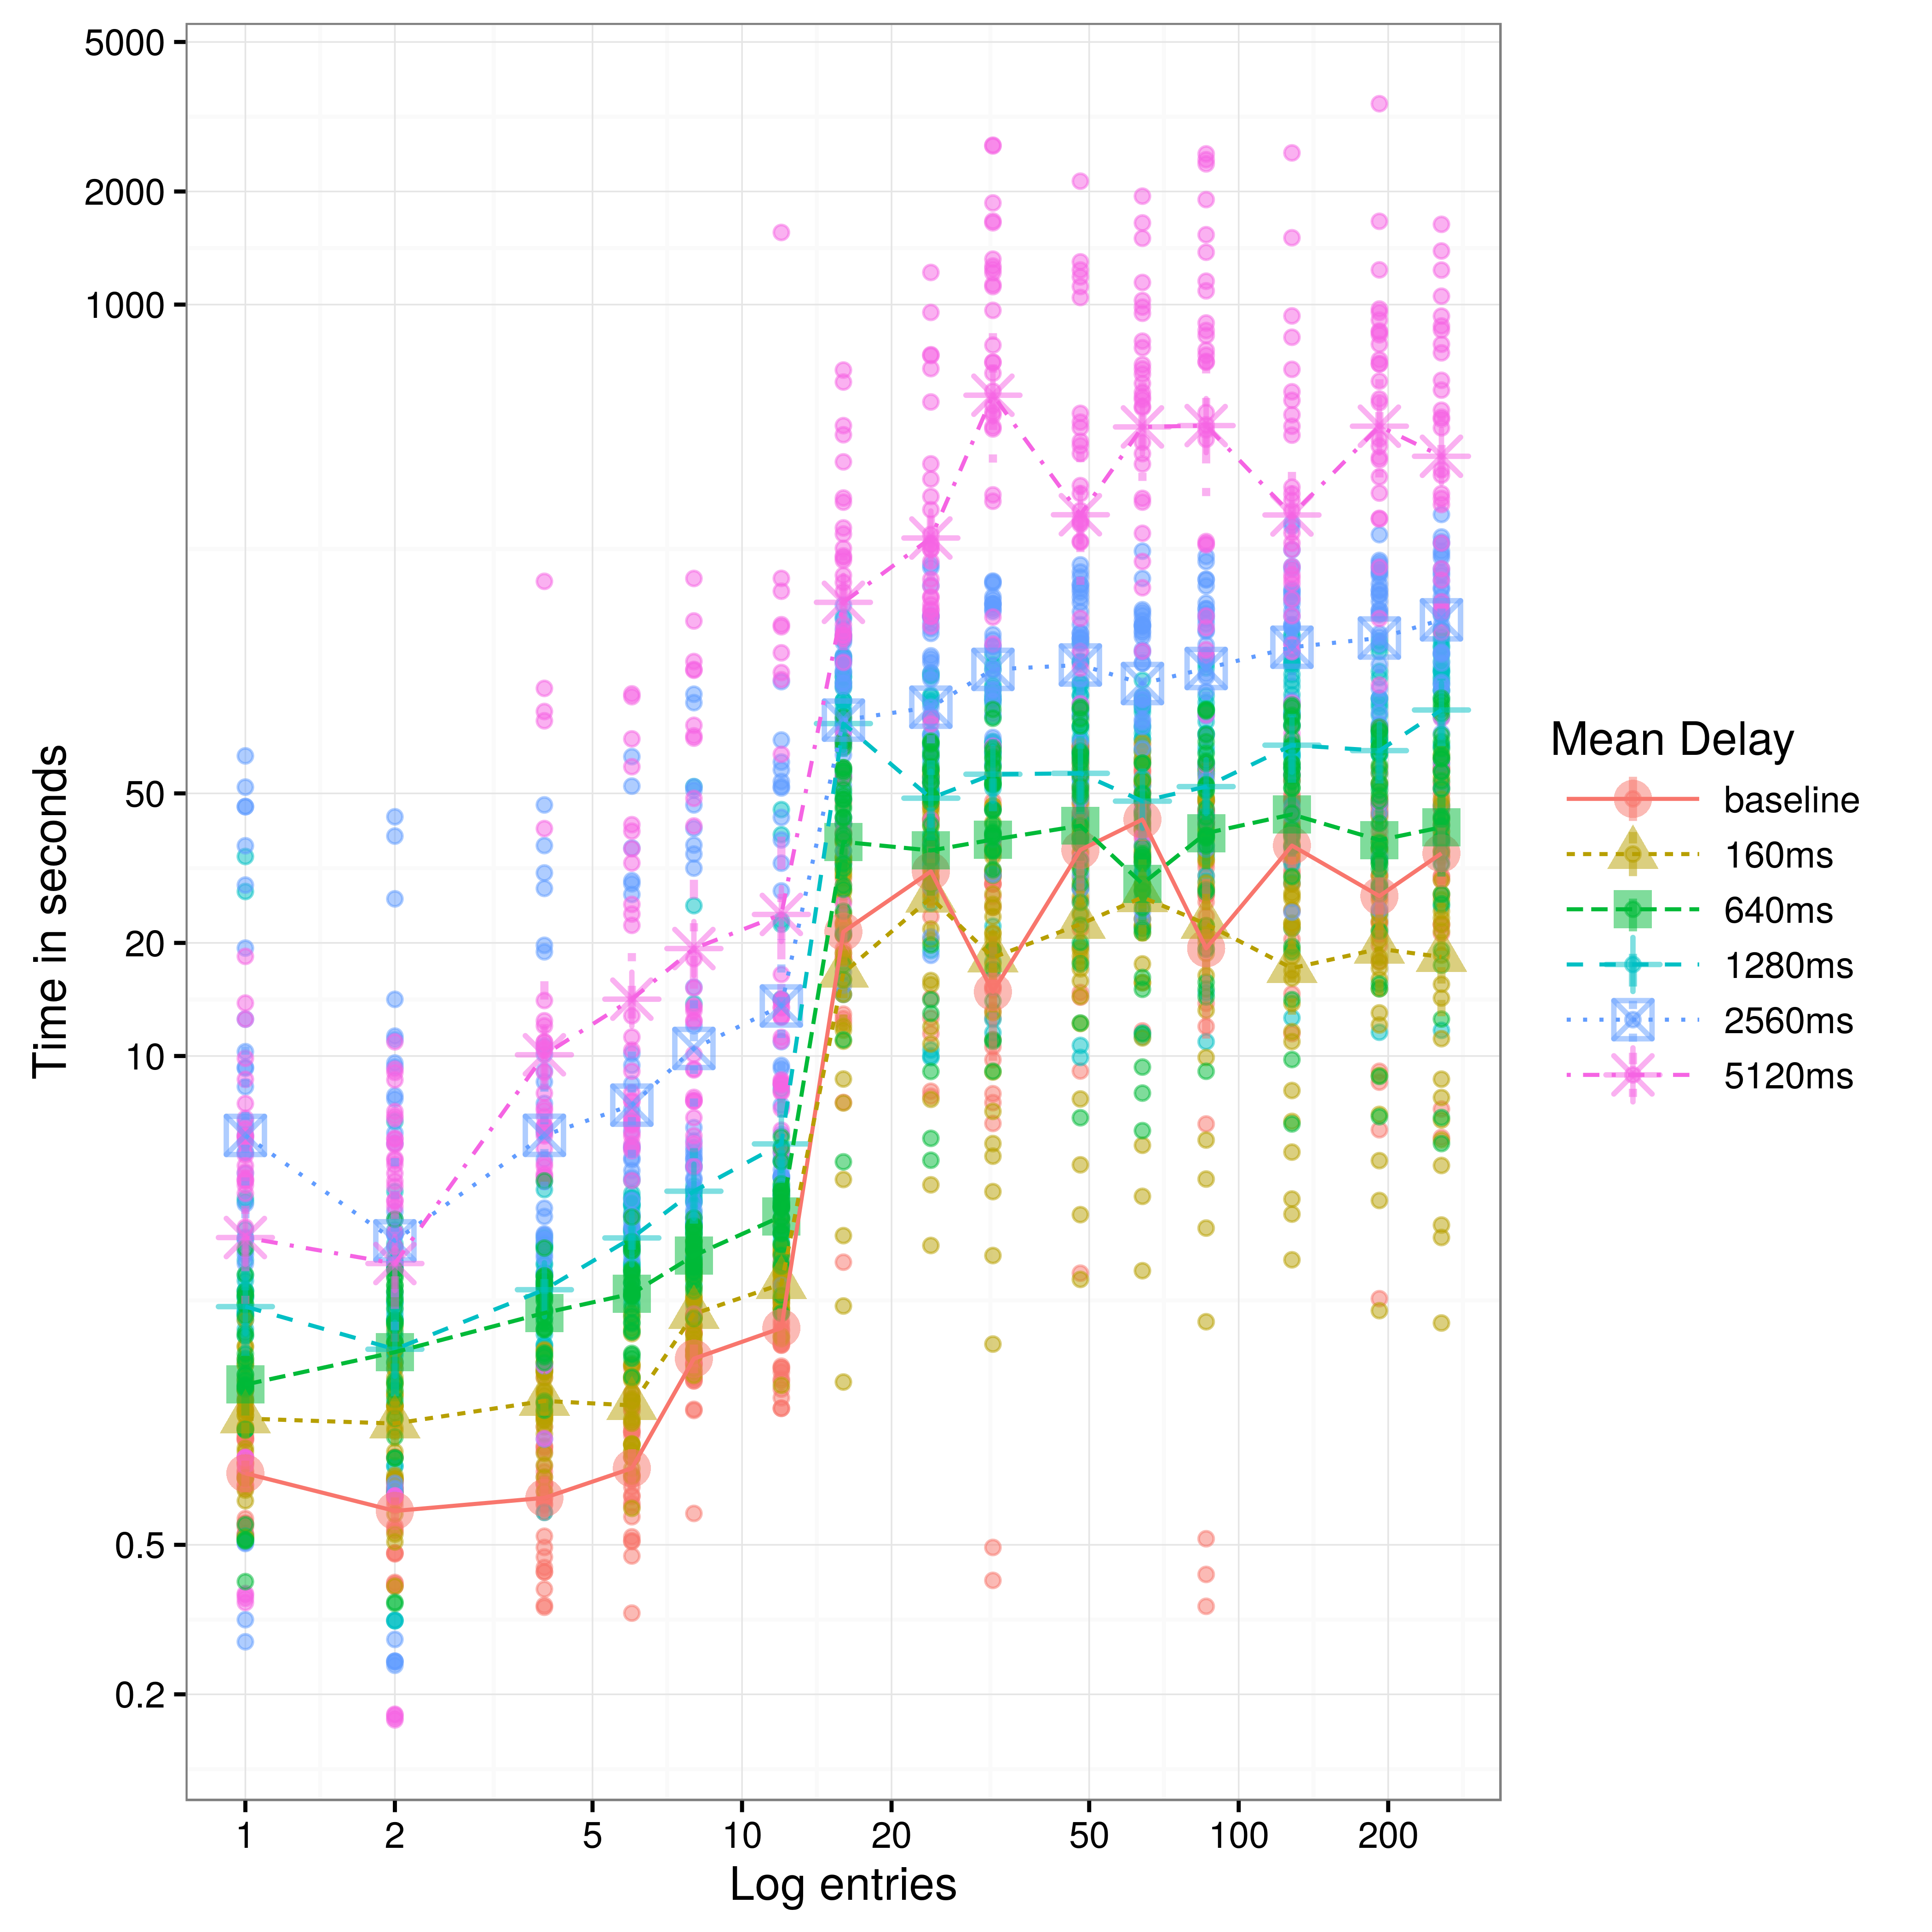
\includegraphics[width=\columnwidth]{imgs/basefs-delay.png}
\caption{BaseFS under variable delay}
\label{fig:basefs-delay}
\end{figure}


Serf is configured to use the WAN profile with a \texttt{ProbeTimeout} of 3 seconds, causing nodes to be reported as failed under latencies greater than 3 seconds. Because of the probabilistic properties of the normal distribution Serf is reporting failed nodes starting from 1280 ms mean delays, seriously impacting BaseFS convergence time. However, the group is able to converge even with mean delays as large as 5120 ms, given enough time.


\subsubsection{Packet Loss Effects}

Figure \ref{fig:basefs-loss} plots the measured convergence time under different packet loss conditions. Increments of 10\% packet loss with 25\% of constant correlation are emulated with \texttt{TC netem}. For example, \texttt{netem loss 30\% 25\%} causes 30\% of packets to be lost, and each successive probability depends by a quarter on the last one. This probability is formally defined as:

$P_n = .25 * P_n-1 + .75 * Random$


% \begin{figure}
% \centering
% 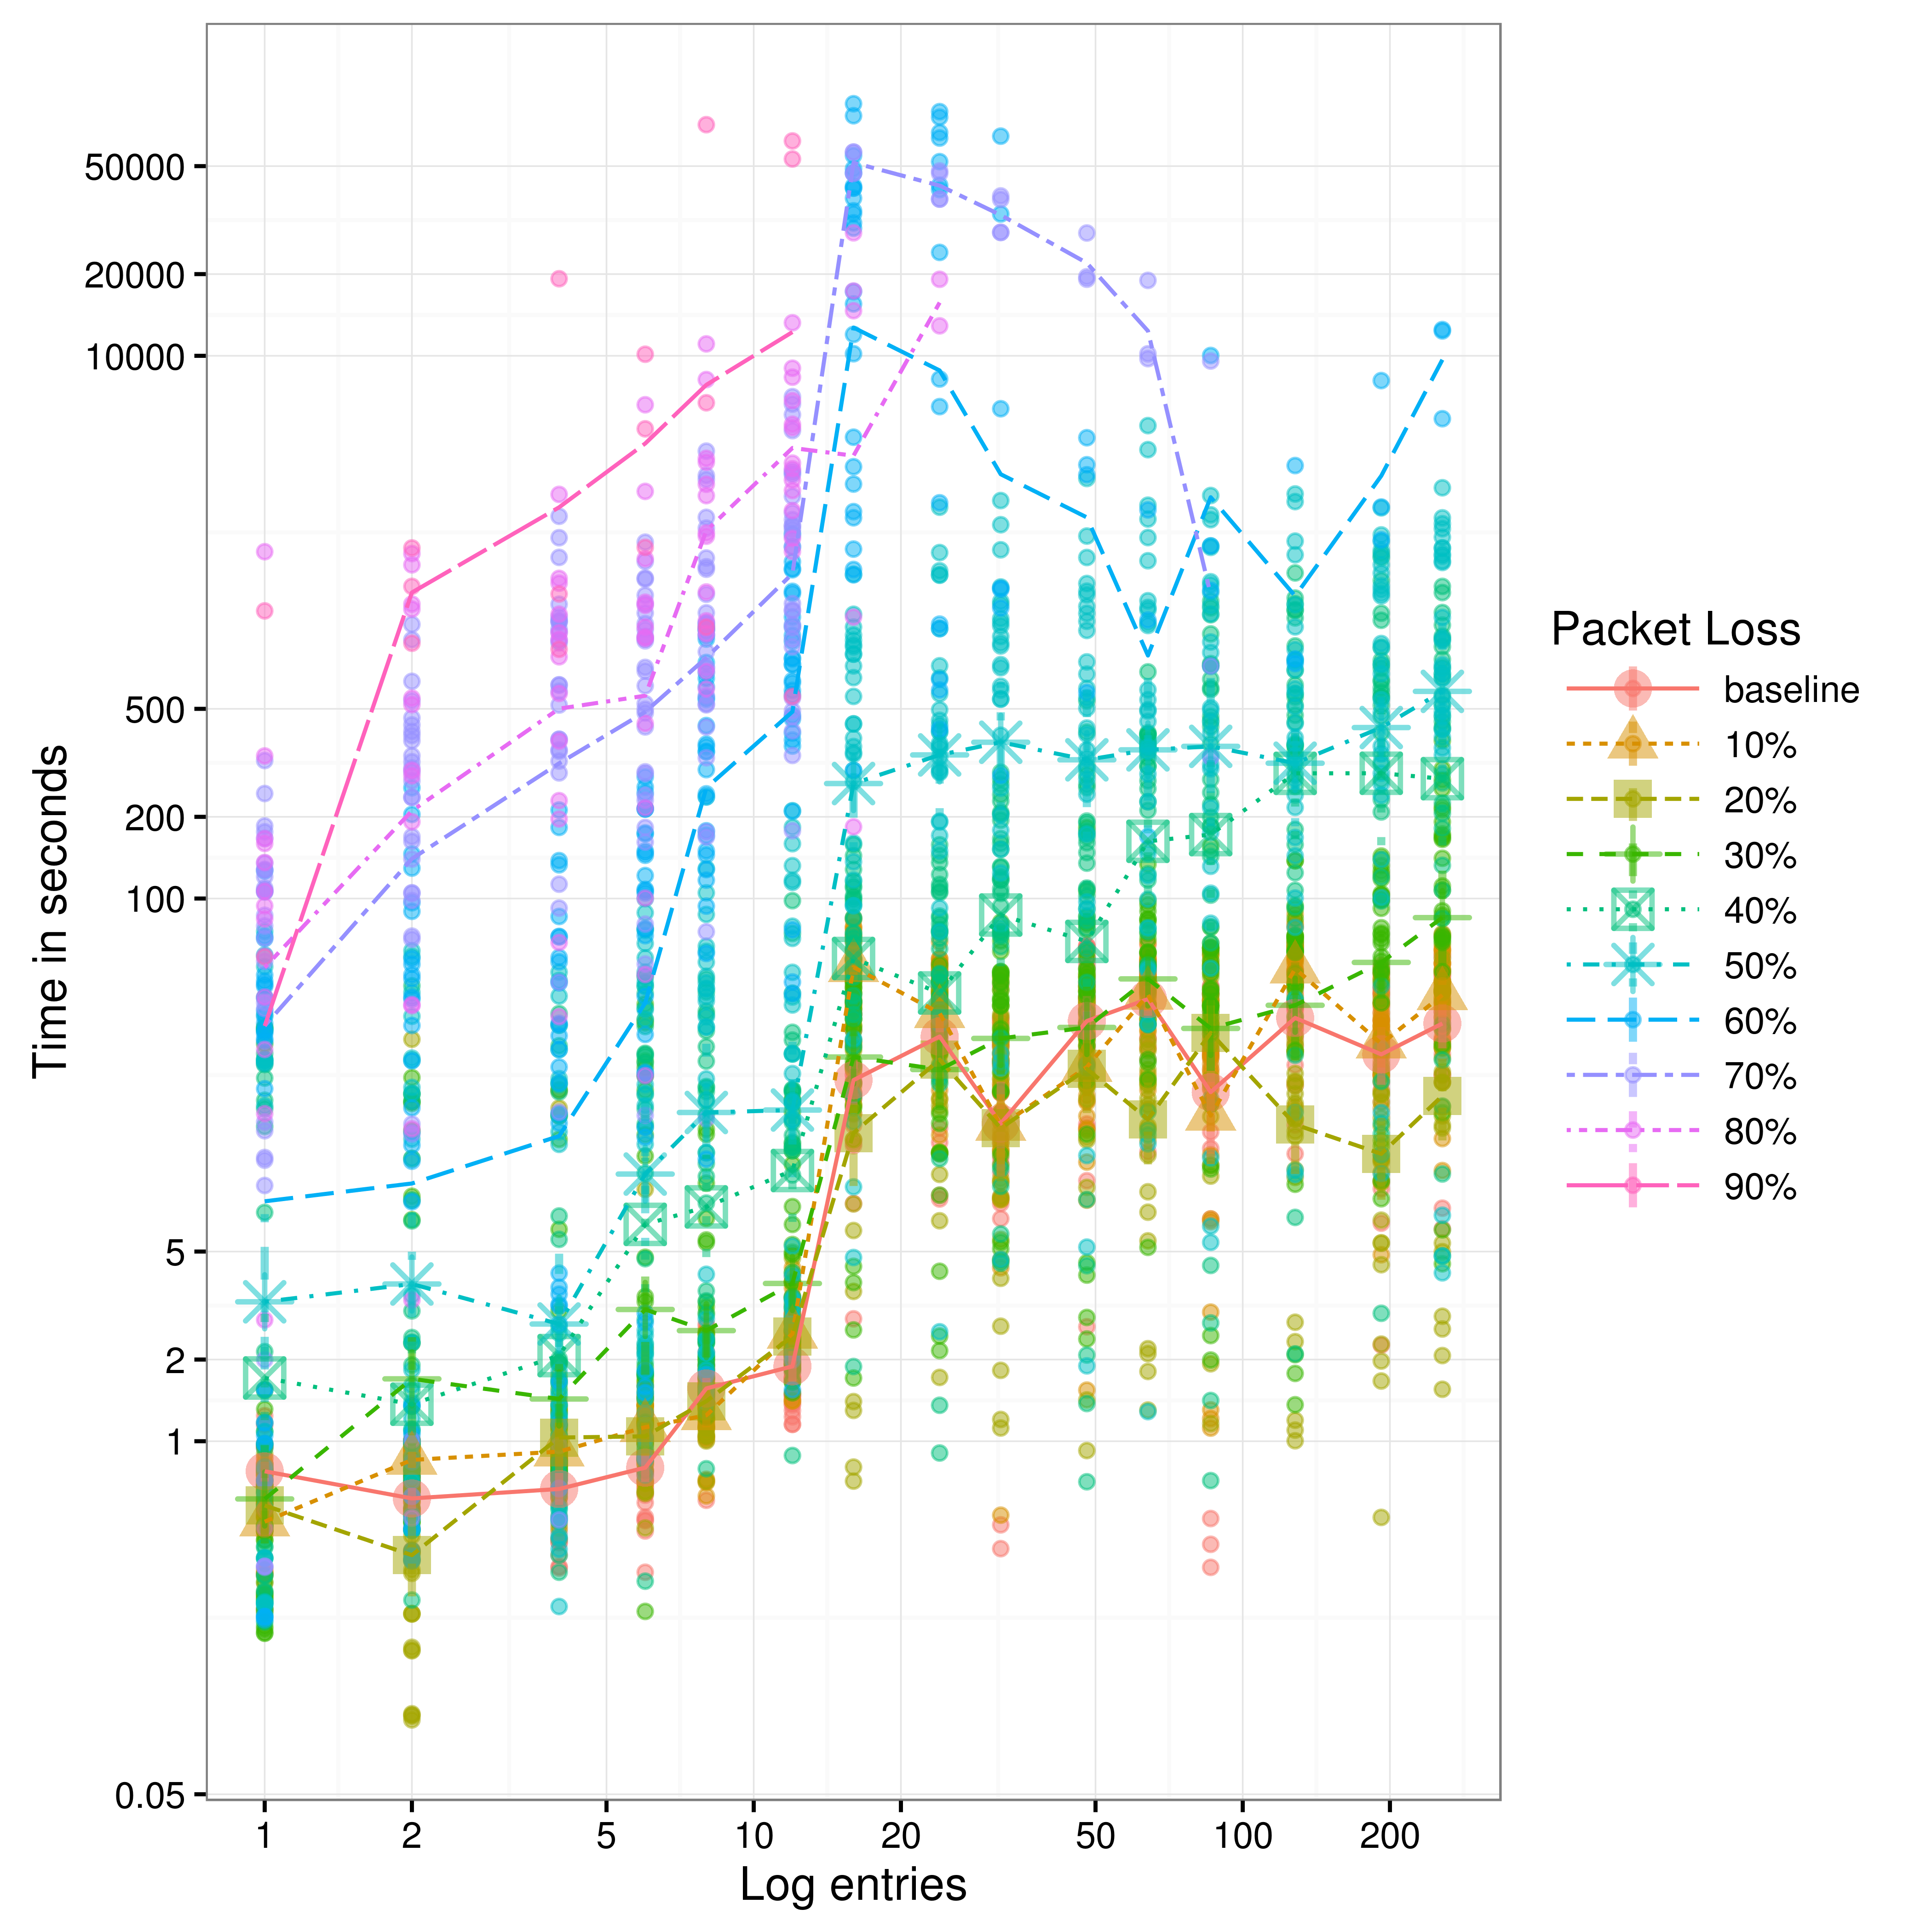
\includegraphics[width=\columnwidth]{imgs/basefs-loss.png}
% \caption{BaseFS under variable packet loss}
% \label{fig:basefs-loss}
% \end{figure}

\begin{figure}
\centering
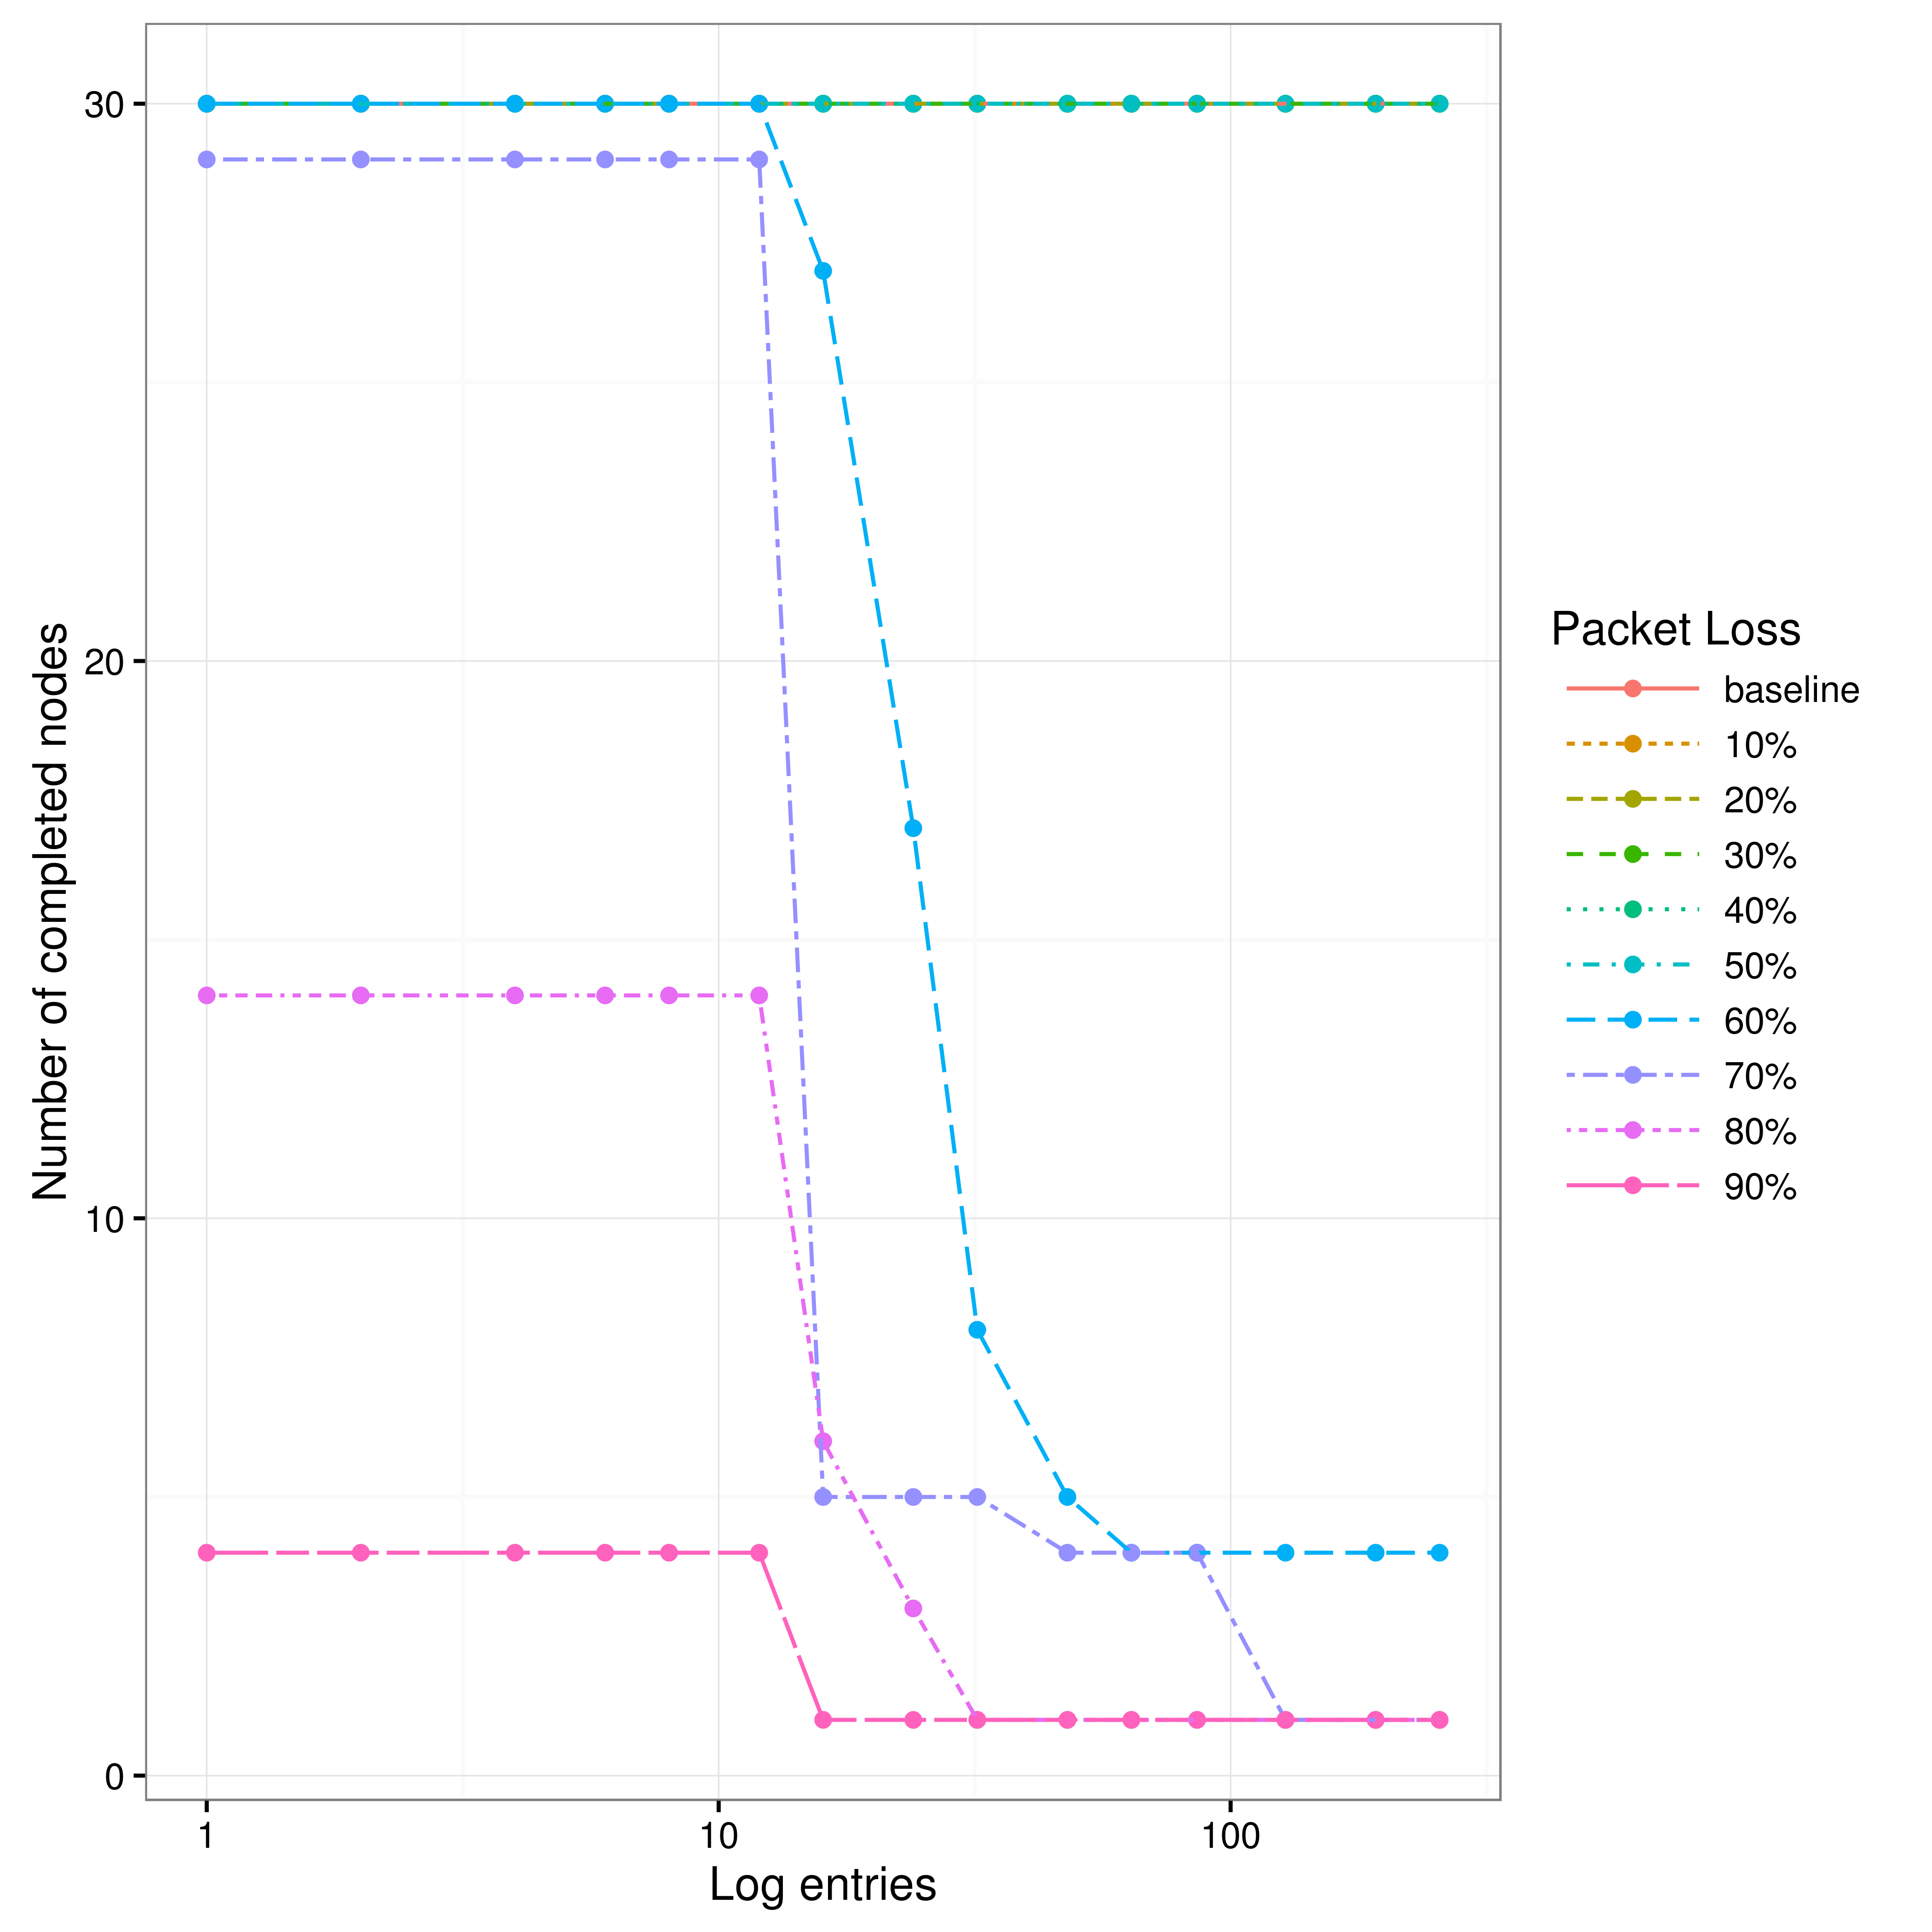
\includegraphics[width=\columnwidth]{imgs/basefs-loss-completed.png}
\caption{BaseFS completed nodes under variable packet loss}
\label{fig:basefs-loss-completed}
\end{figure}


Serf WAN profile sets \texttt{GossipNodes} to 4 nodes, causing messages to be gossiped only to 4 random peers. Gossip messages are transported over UDP, without retransmission. Lost messages causes the gossip layer to report nodes as failed, also affecting the synchronization protocol, since only alive nodes are contacted. 0.5 chance of packet loss is the tipping point where the system fails to converge. Particularly when block dissemination is not performed by the gossip layer (more than 10 blocks). In this case the number of gossiped messages is not enough to sustained a reliable group member list, and the system rapidly degrades as time passes. By increasing Serf's \texttt{GossipNodes} and tunning \texttt{SuspicionMult} and \texttt{IndirectChecks} we can improve the chances of successful gossip messages delivery and the chances of detecting alive nodes, alleviating the substantial effects produced by heavy packet loss conditions.


\subsubsection{Bandwidth Limitations Effects}

Figure \ref{fig:basefs-bw} shows the measured convergence time of several operations on different bandwidth constrained settings. Hierarchical Token Buckets (HTB) queuing discipline is used to emulate various link data rates, for example \texttt{htb rate 32kbit}.

\begin{figure}
\centering
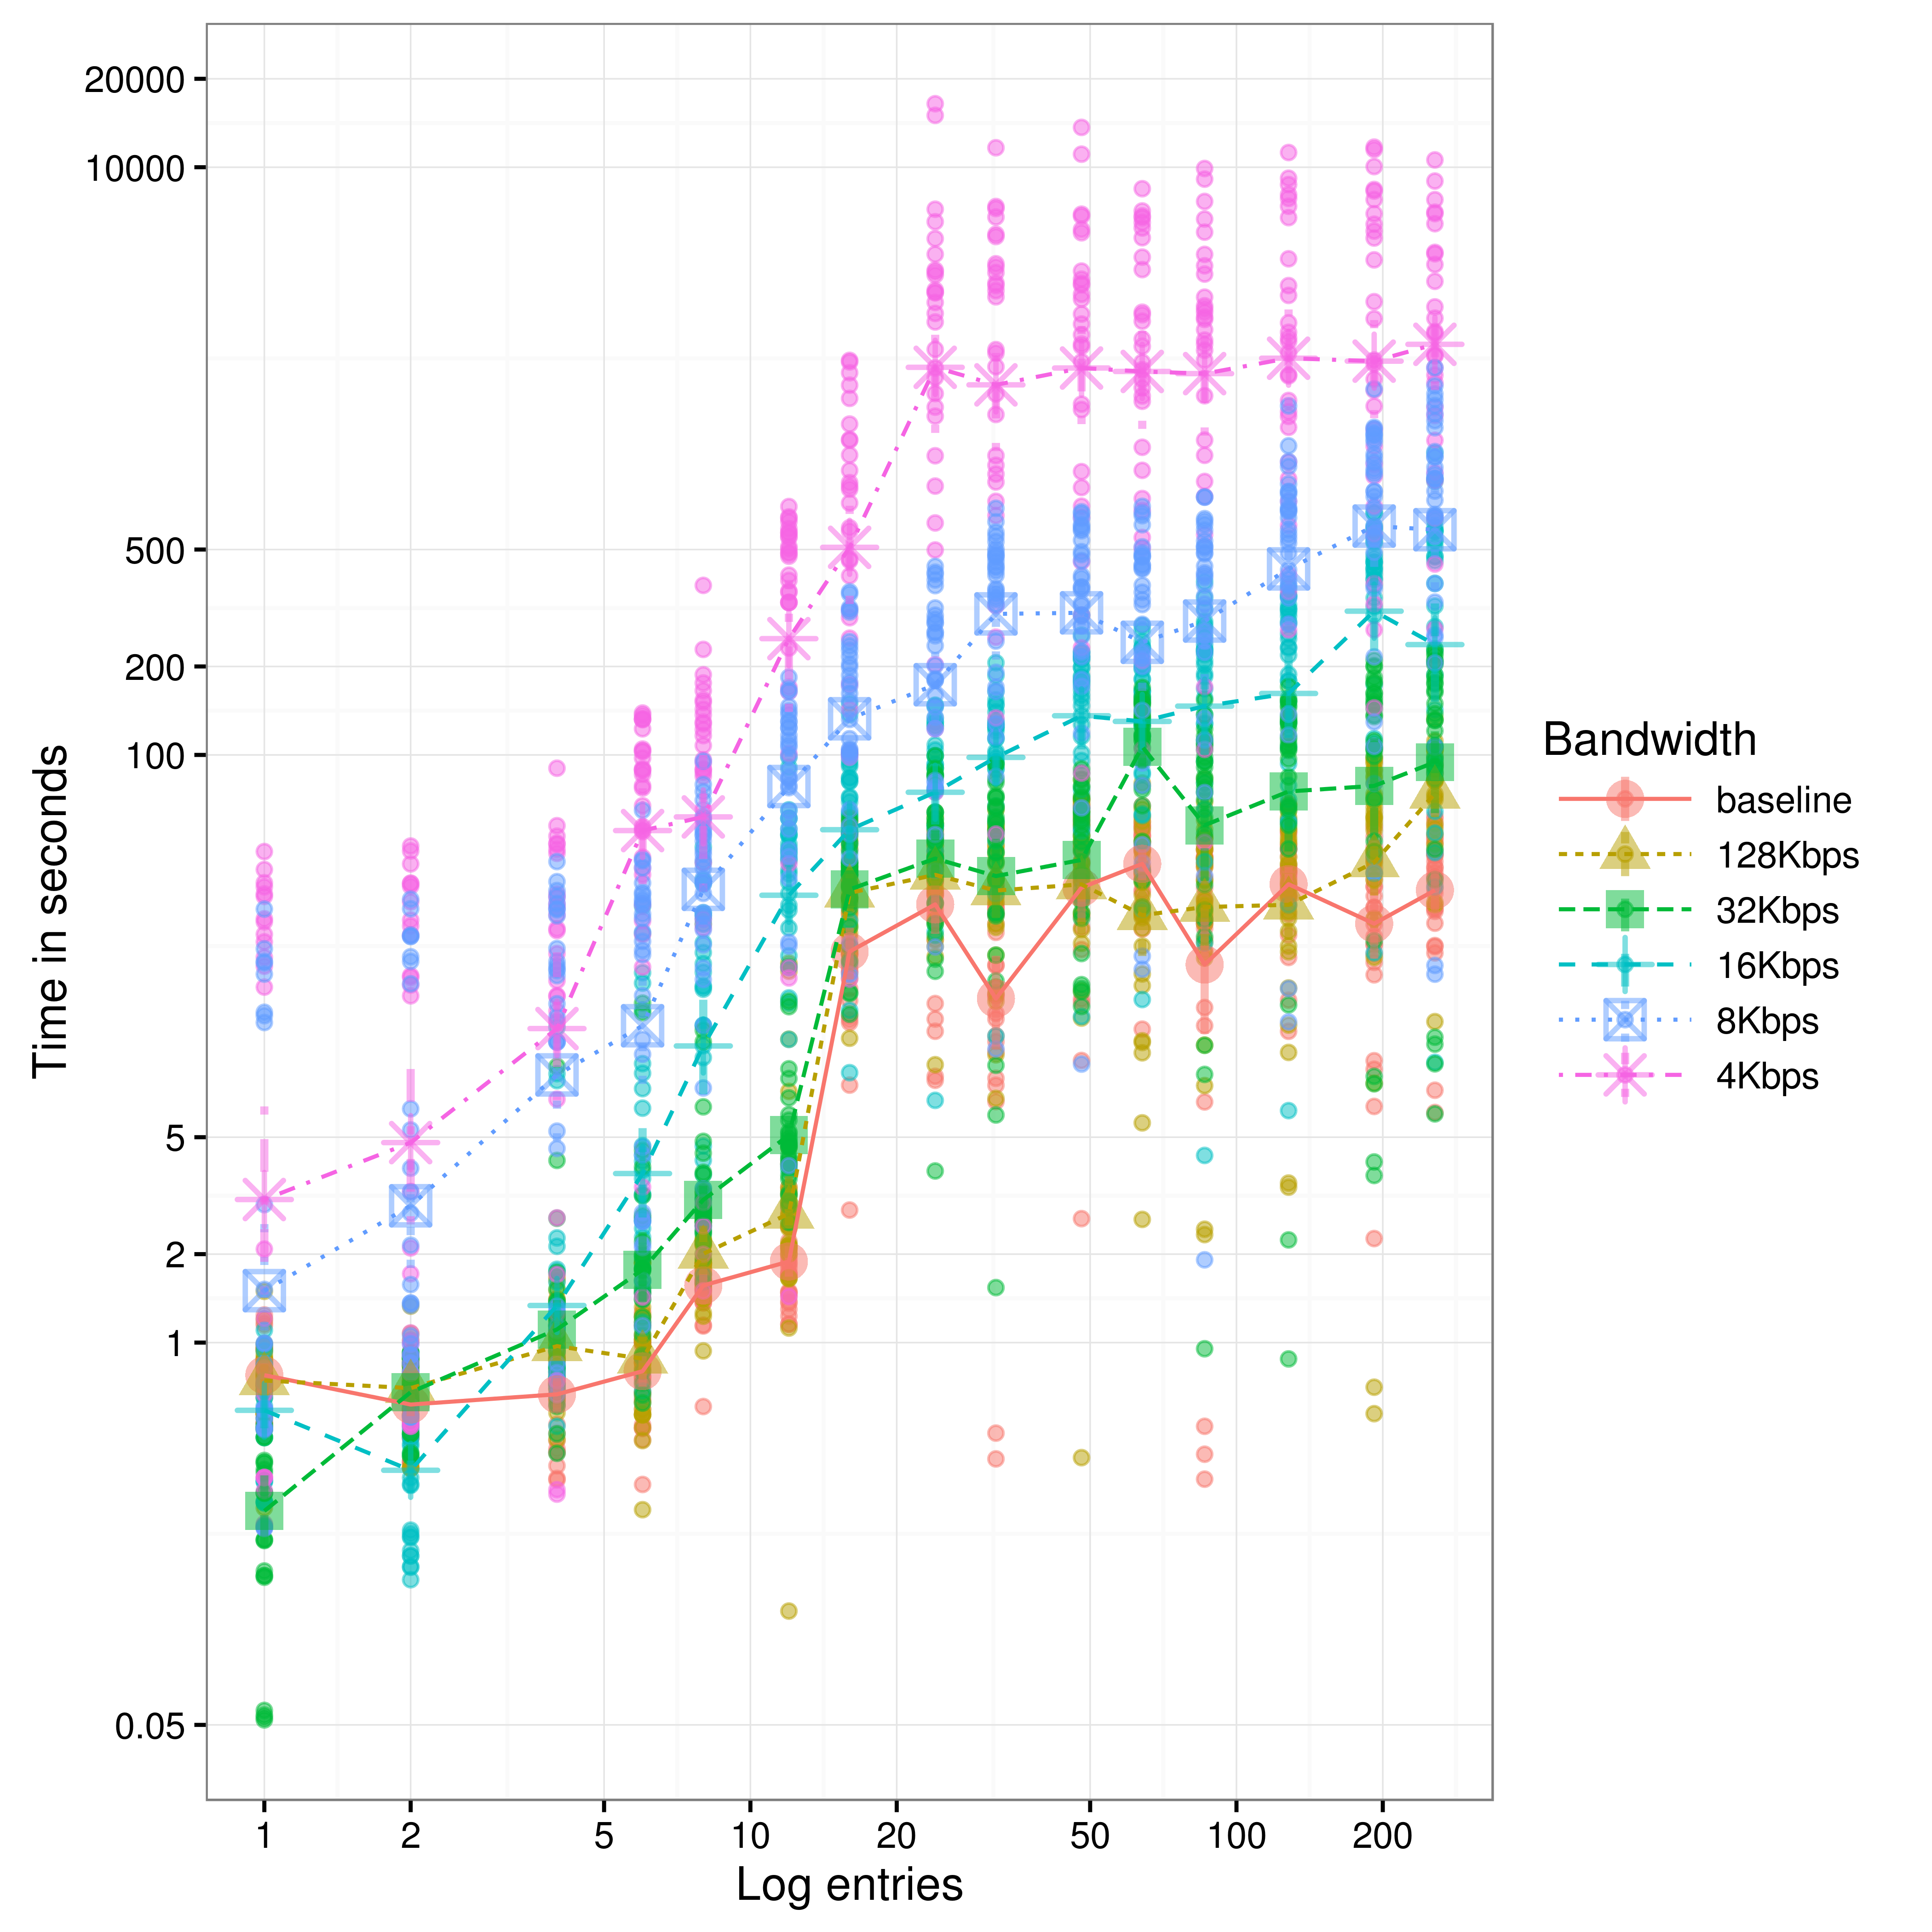
\includegraphics[width=\columnwidth]{imgs/basefs-bw.png}
\caption{BaseFS under variable bandwidth}
\label{fig:basefs-bw}
\end{figure}

Our measurements are consistent with Serf's analytical bandwidth estimate\footnote{https://www.serfdom.io/docs/internals/simulator.html} of 175 kbps/node per message. Bandwidth limitations up to 256 kbps do not have significant impact on the convergence time. Even a 32 kbps data rate only produces a 20\% time increase respect to baseline.

\subsubsection{BaseFS Under Community-Lab}

We have instantiated a Community-Lab slice consisting on 35 slivers with public IPv4 connectivity between them. To install required BaseFS dependencies we deployed an APT (Debian package manager) and a PIP (Python package manager) proxies over the management network\footnote{https://wiki.confine-project.eu/arch:management-network}. To ensure all sliver's clocks are properly synchronized we also deployed our NTP server over the management network (NTP traffic is filtered on CONFINE's public network).

Figure \ref{fig:topology} shows the public IPv4 network topology of the 35 node slice, uncovering an unfortunate cluster of 20 nodes connected to the same collision domain. Figure \ref{fig:characterization} shows the hop and latency distributions of the slice.


\begin{figure}
\centering
\includegraphics[width=200pt]{imgs/topology.png}
\caption{Community-Lab slice network topology}
\label{fig:topology}
\end{figure}

Figure \ref{fig:basefs} shows the measured convergence time of a simulated workload on Community-Lab. The workload consists on 560 writes. 60\% of which produce one log entry, 28\% 2 entries and 3, 5 and 17 entries are produced 3.5\% of the time each. The experiment is replicated using Docker containers for reference.


\begin{figure}
\centering
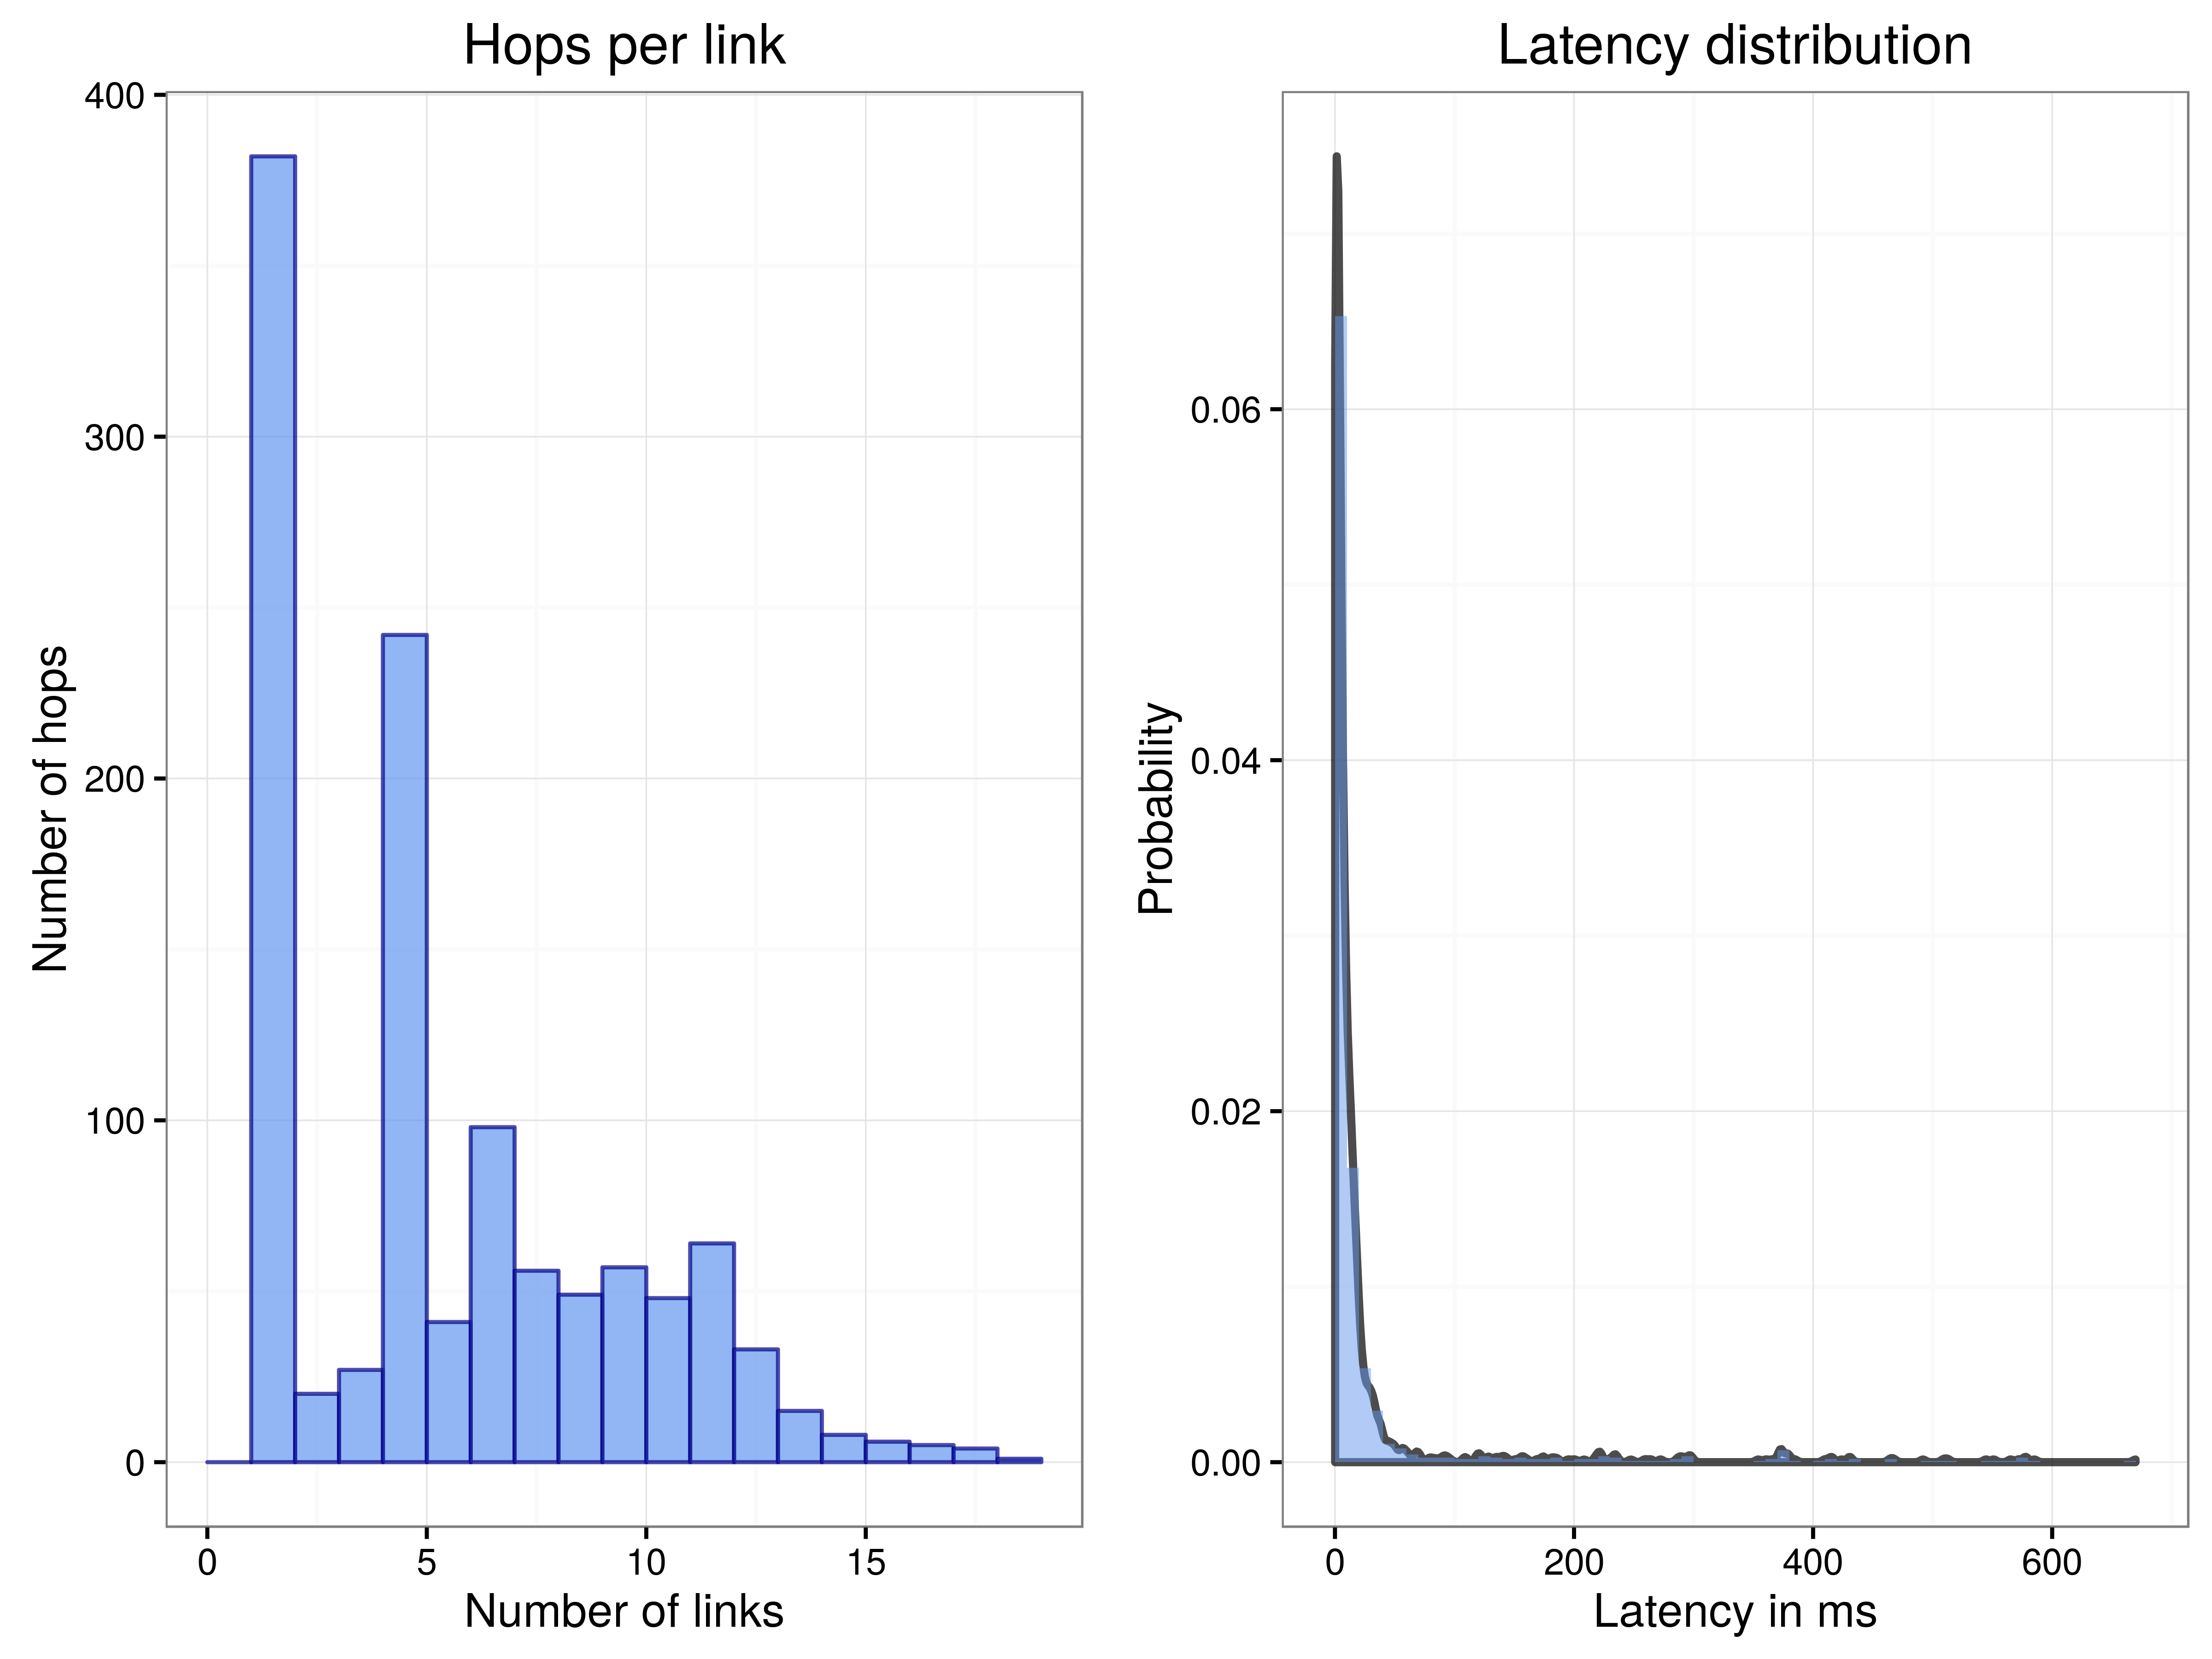
\includegraphics[width=\columnwidth]{imgs/characterization.png}
\caption{Community-Lab slice characterization}
\label{fig:characterization}
\end{figure}


\begin{figure}
\centering
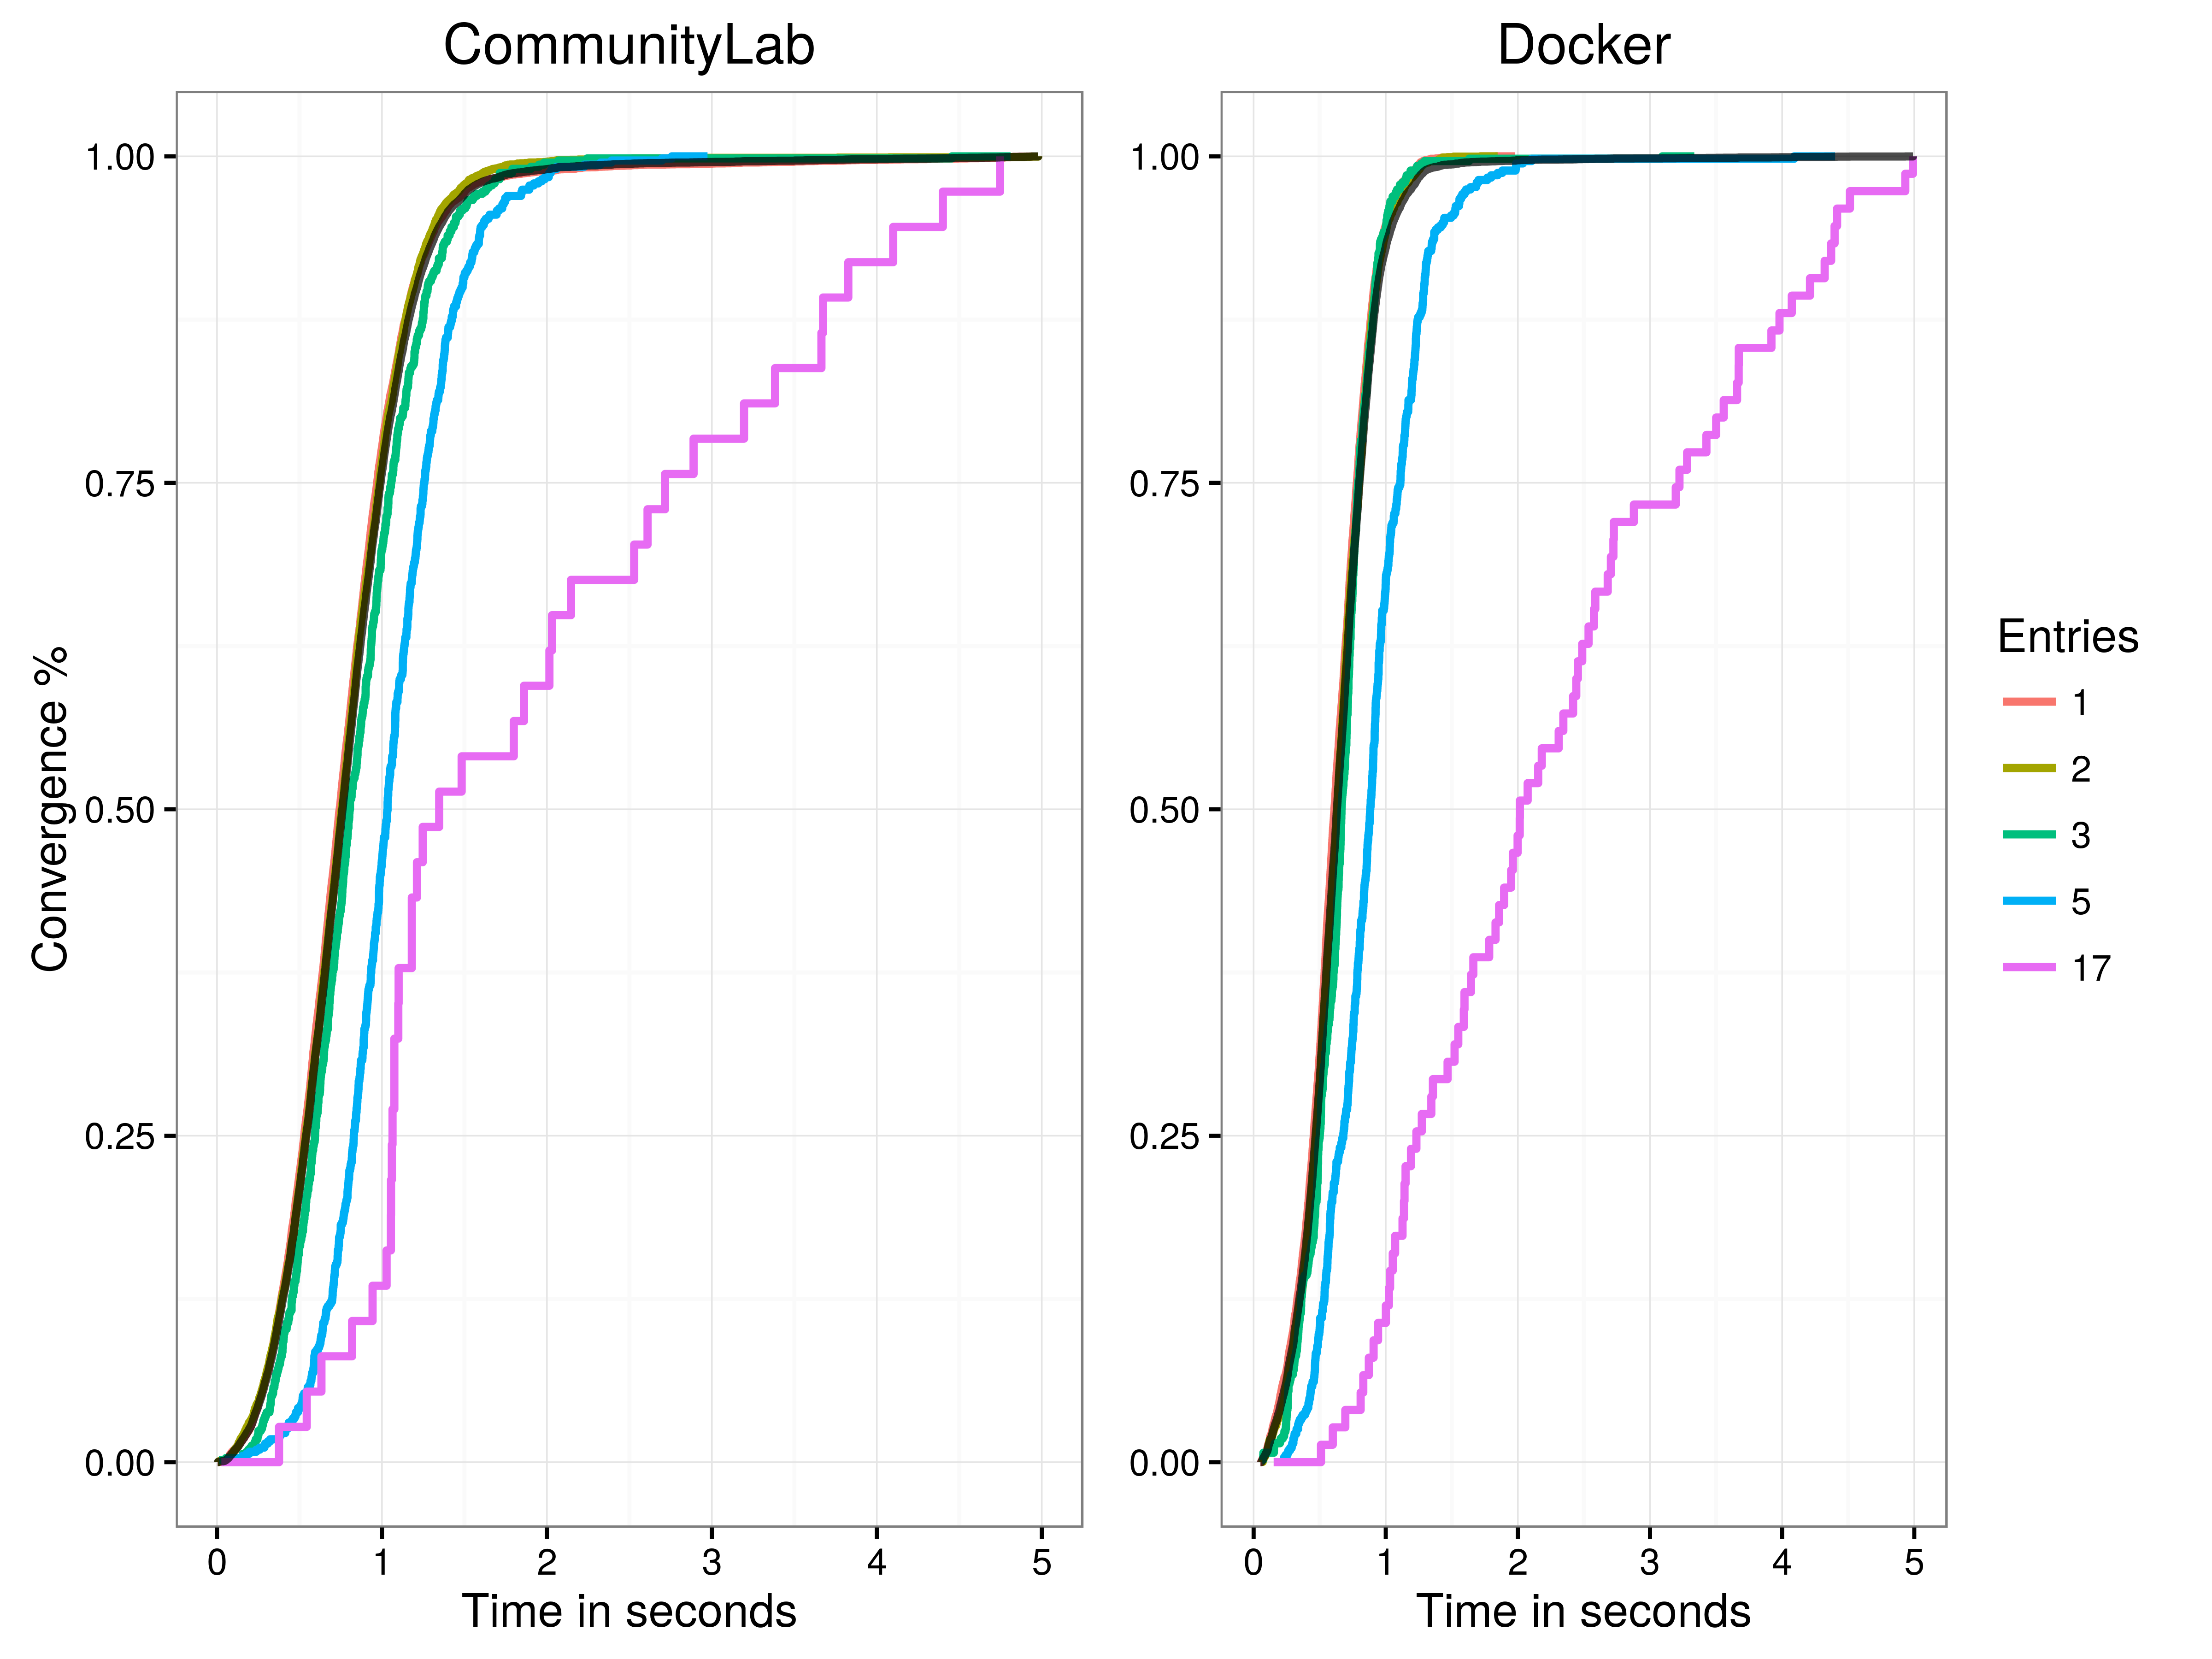
\includegraphics[width=\columnwidth]{imgs/basefs.png}
\caption{BaseFS convergence time}
\label{fig:basefs}
\end{figure}


\begin{figure}
\centering
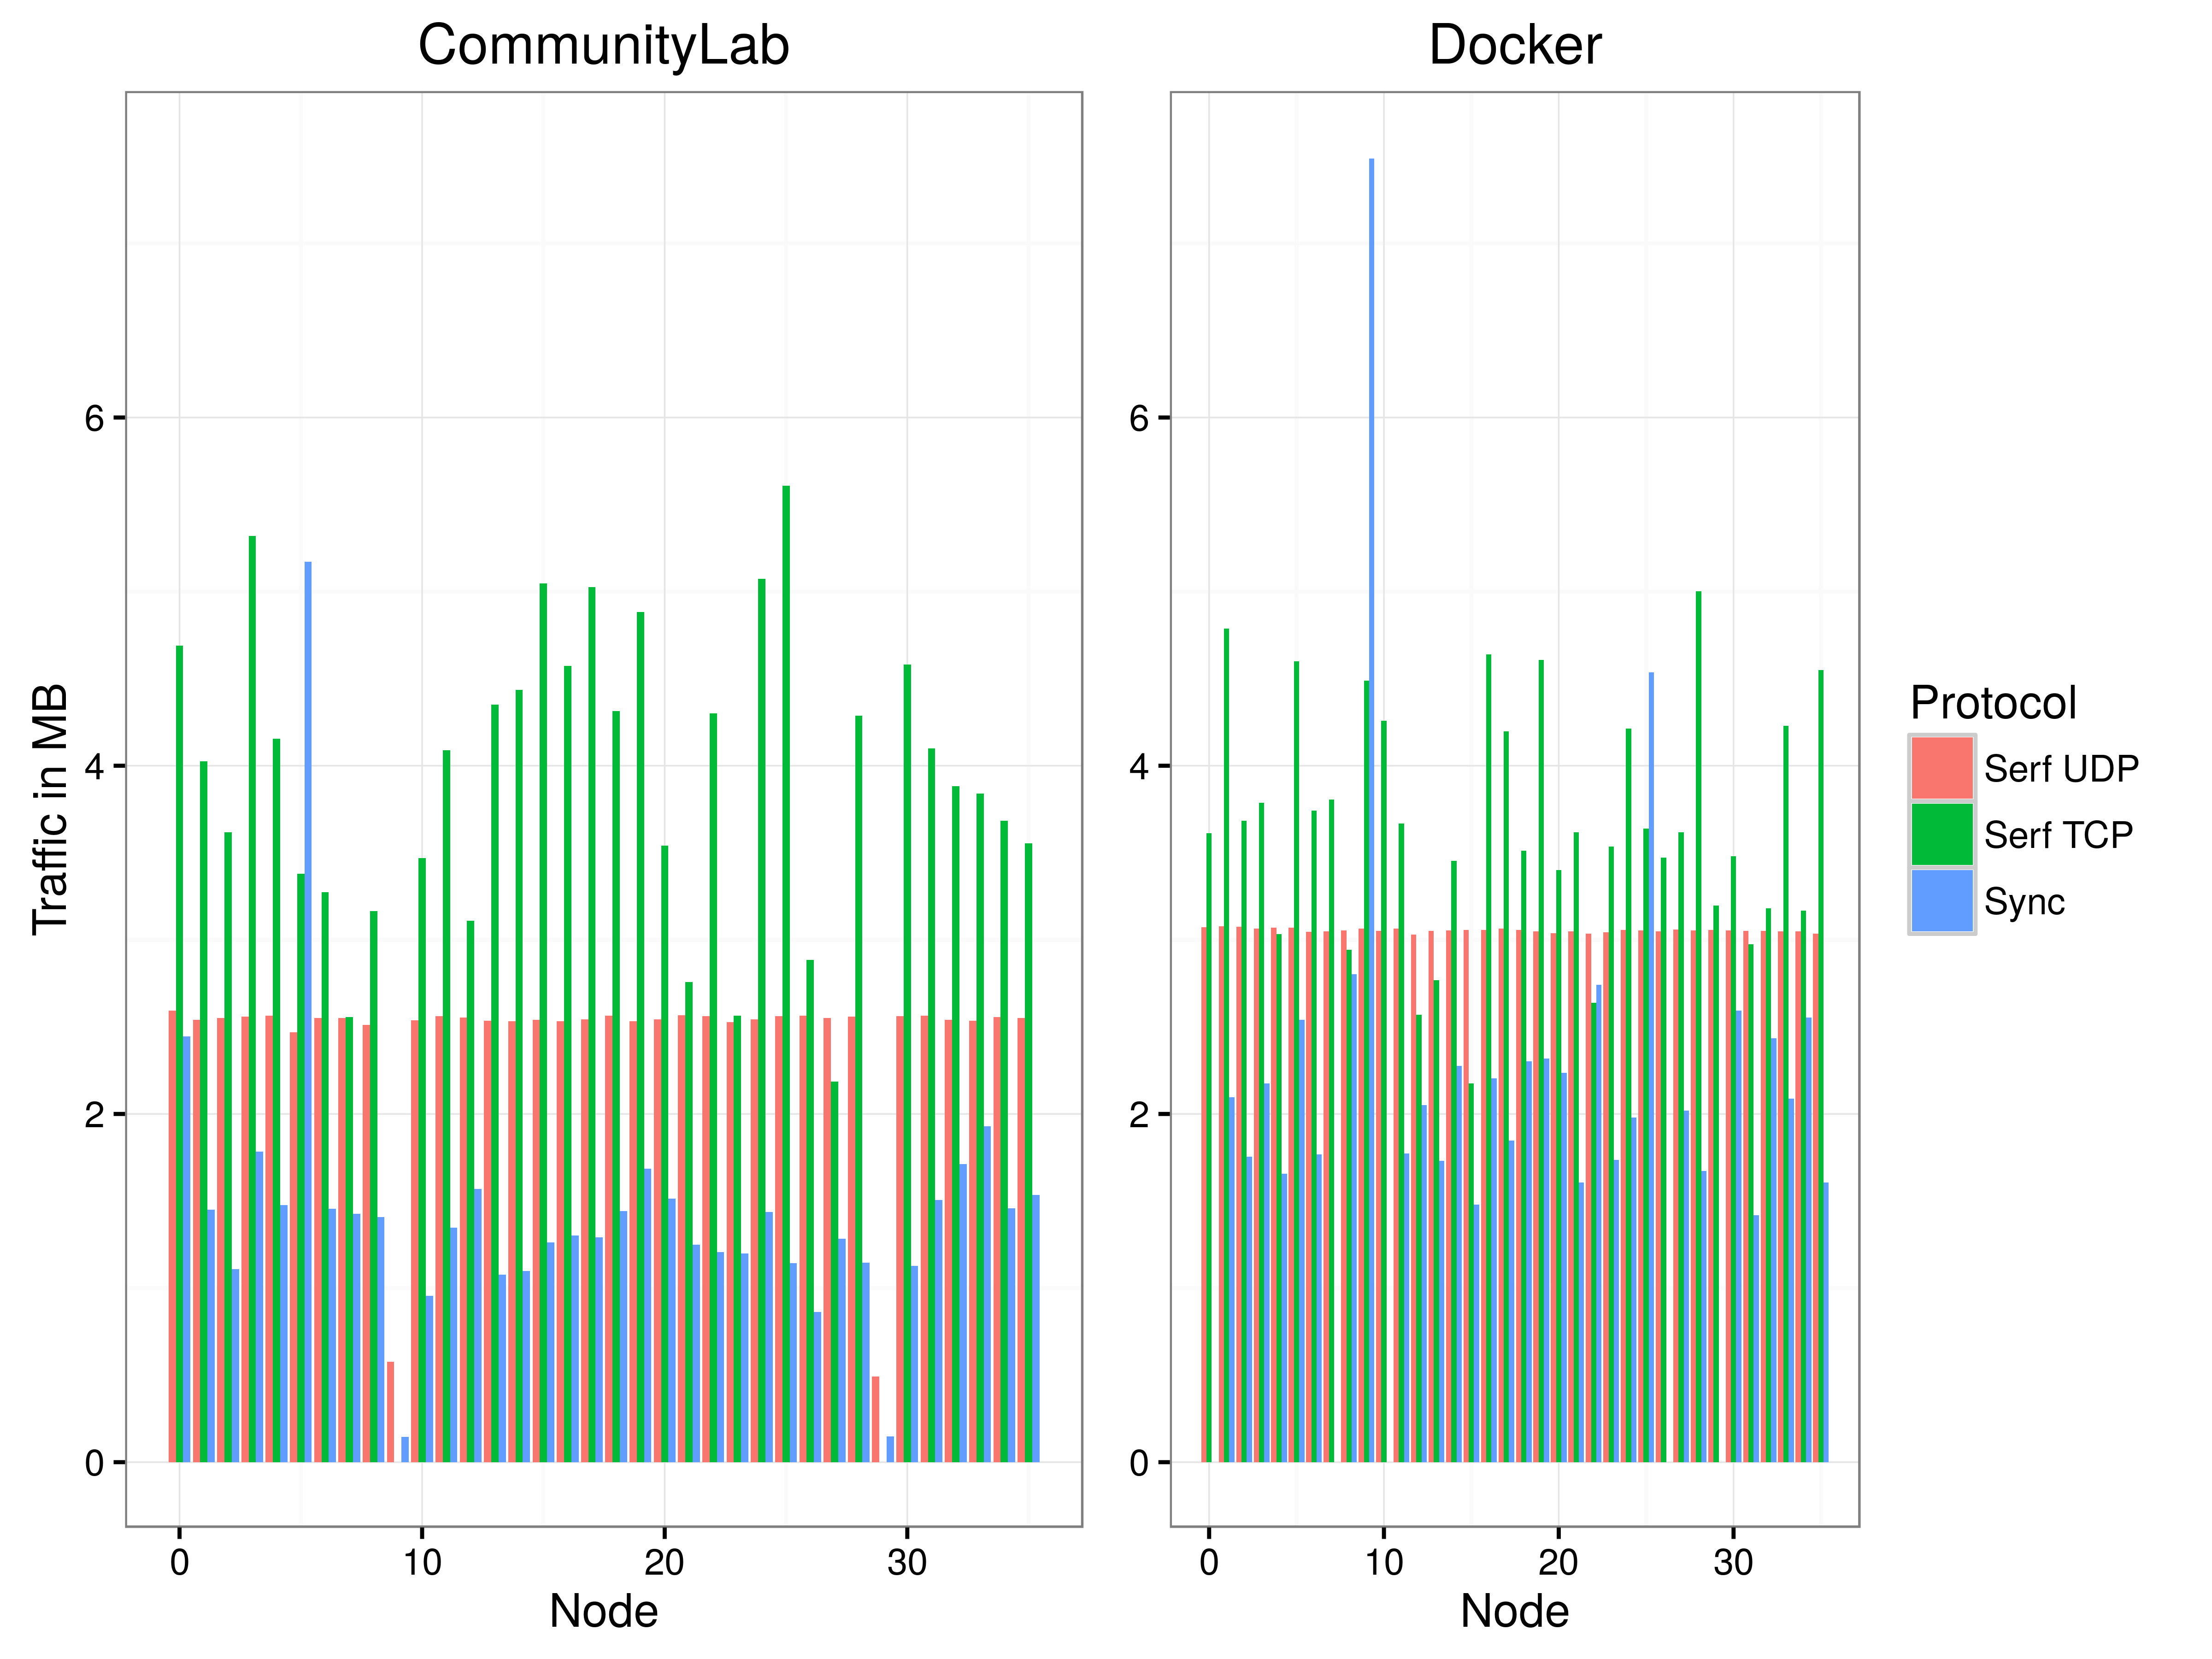
\includegraphics[width=\columnwidth]{imgs/basefs-traffic-distribution.png}
\caption{BaseFS outgoing traffic distribution}
\label{fig:basefs-traffic-distribution}
\end{figure}


An evenly distributed traffic consumption throughout the members is a quality expected from any peer-to-peer system. Figure \ref{fig:basefs-traffic-distribution} shows the outgoing traffic distribution measured during the experiment. The poor traffic contributions of nodes 9 and 29 are due to an error on Community-Lab testbed. Both nodes did not receive a public IP address, but a private one, lagging behind a NAT. Contact initiated by other nodes is not possible, but NATed nodes can still receive log entries by means of the sync protocol. We didn't intend to have NATed nodes, but this brings the opportunity to validate that BaseFS can deal with an small number of them. At this point we can not determine if the differences on performance between Community-Lab and Docker are due to the NATed nodes or other factors.



\subsection{File Operations Performance}
    
In this section we compare BaseFS to a more traditional filesystem (EXT4). The experiments roughly show how file updates affect read and write performance at the filesystem level, while having a known filesystem like EXT4 to help putting results into perspective. The experiment consists on copying up to 30 times the entire content of the \texttt{/etc} root directory (files, directories and symbolic links), a workload designed to hurt Basefs Bsdiff4 usage. Notice that this performance test only involves a single node, the performance of a group is the aggregated IO from all the nodes.

The \texttt{/etc} directory of the testing machine contained:

\begin{itemize}
 \item 2512 files
 \item 1350 symbolic links
 \item 462 directories
 \item 22 MB of data
\end{itemize}

Bear in mind that we are comparing a kernelspace filesystem (EXT4) with a userspace virtual filesystem that requires executing complex algorithms on top of cPyhton, with the additional FUSE layer and the added cost of having to context switch into kernel mode for performing system calls.

\subsubsection{Read Performance}

Starting from a fresh log file, the entire \texttt{/etc} directory is recursively copied into BaseFS mounted directory on each round. Then two reads are performed, the first has to compute the binary difference of every previous version, but the second is cached. We do the same with an EXT4 filesystem stored on a SATA drive. In this case, however, we perform a \texttt{sync \&\& echo 3 > /proc/sys/vm/drop\_caches} after every write i order to clean any possible caching and do the first read as cold as the BaseFS one.

\begin{figure}
\centering
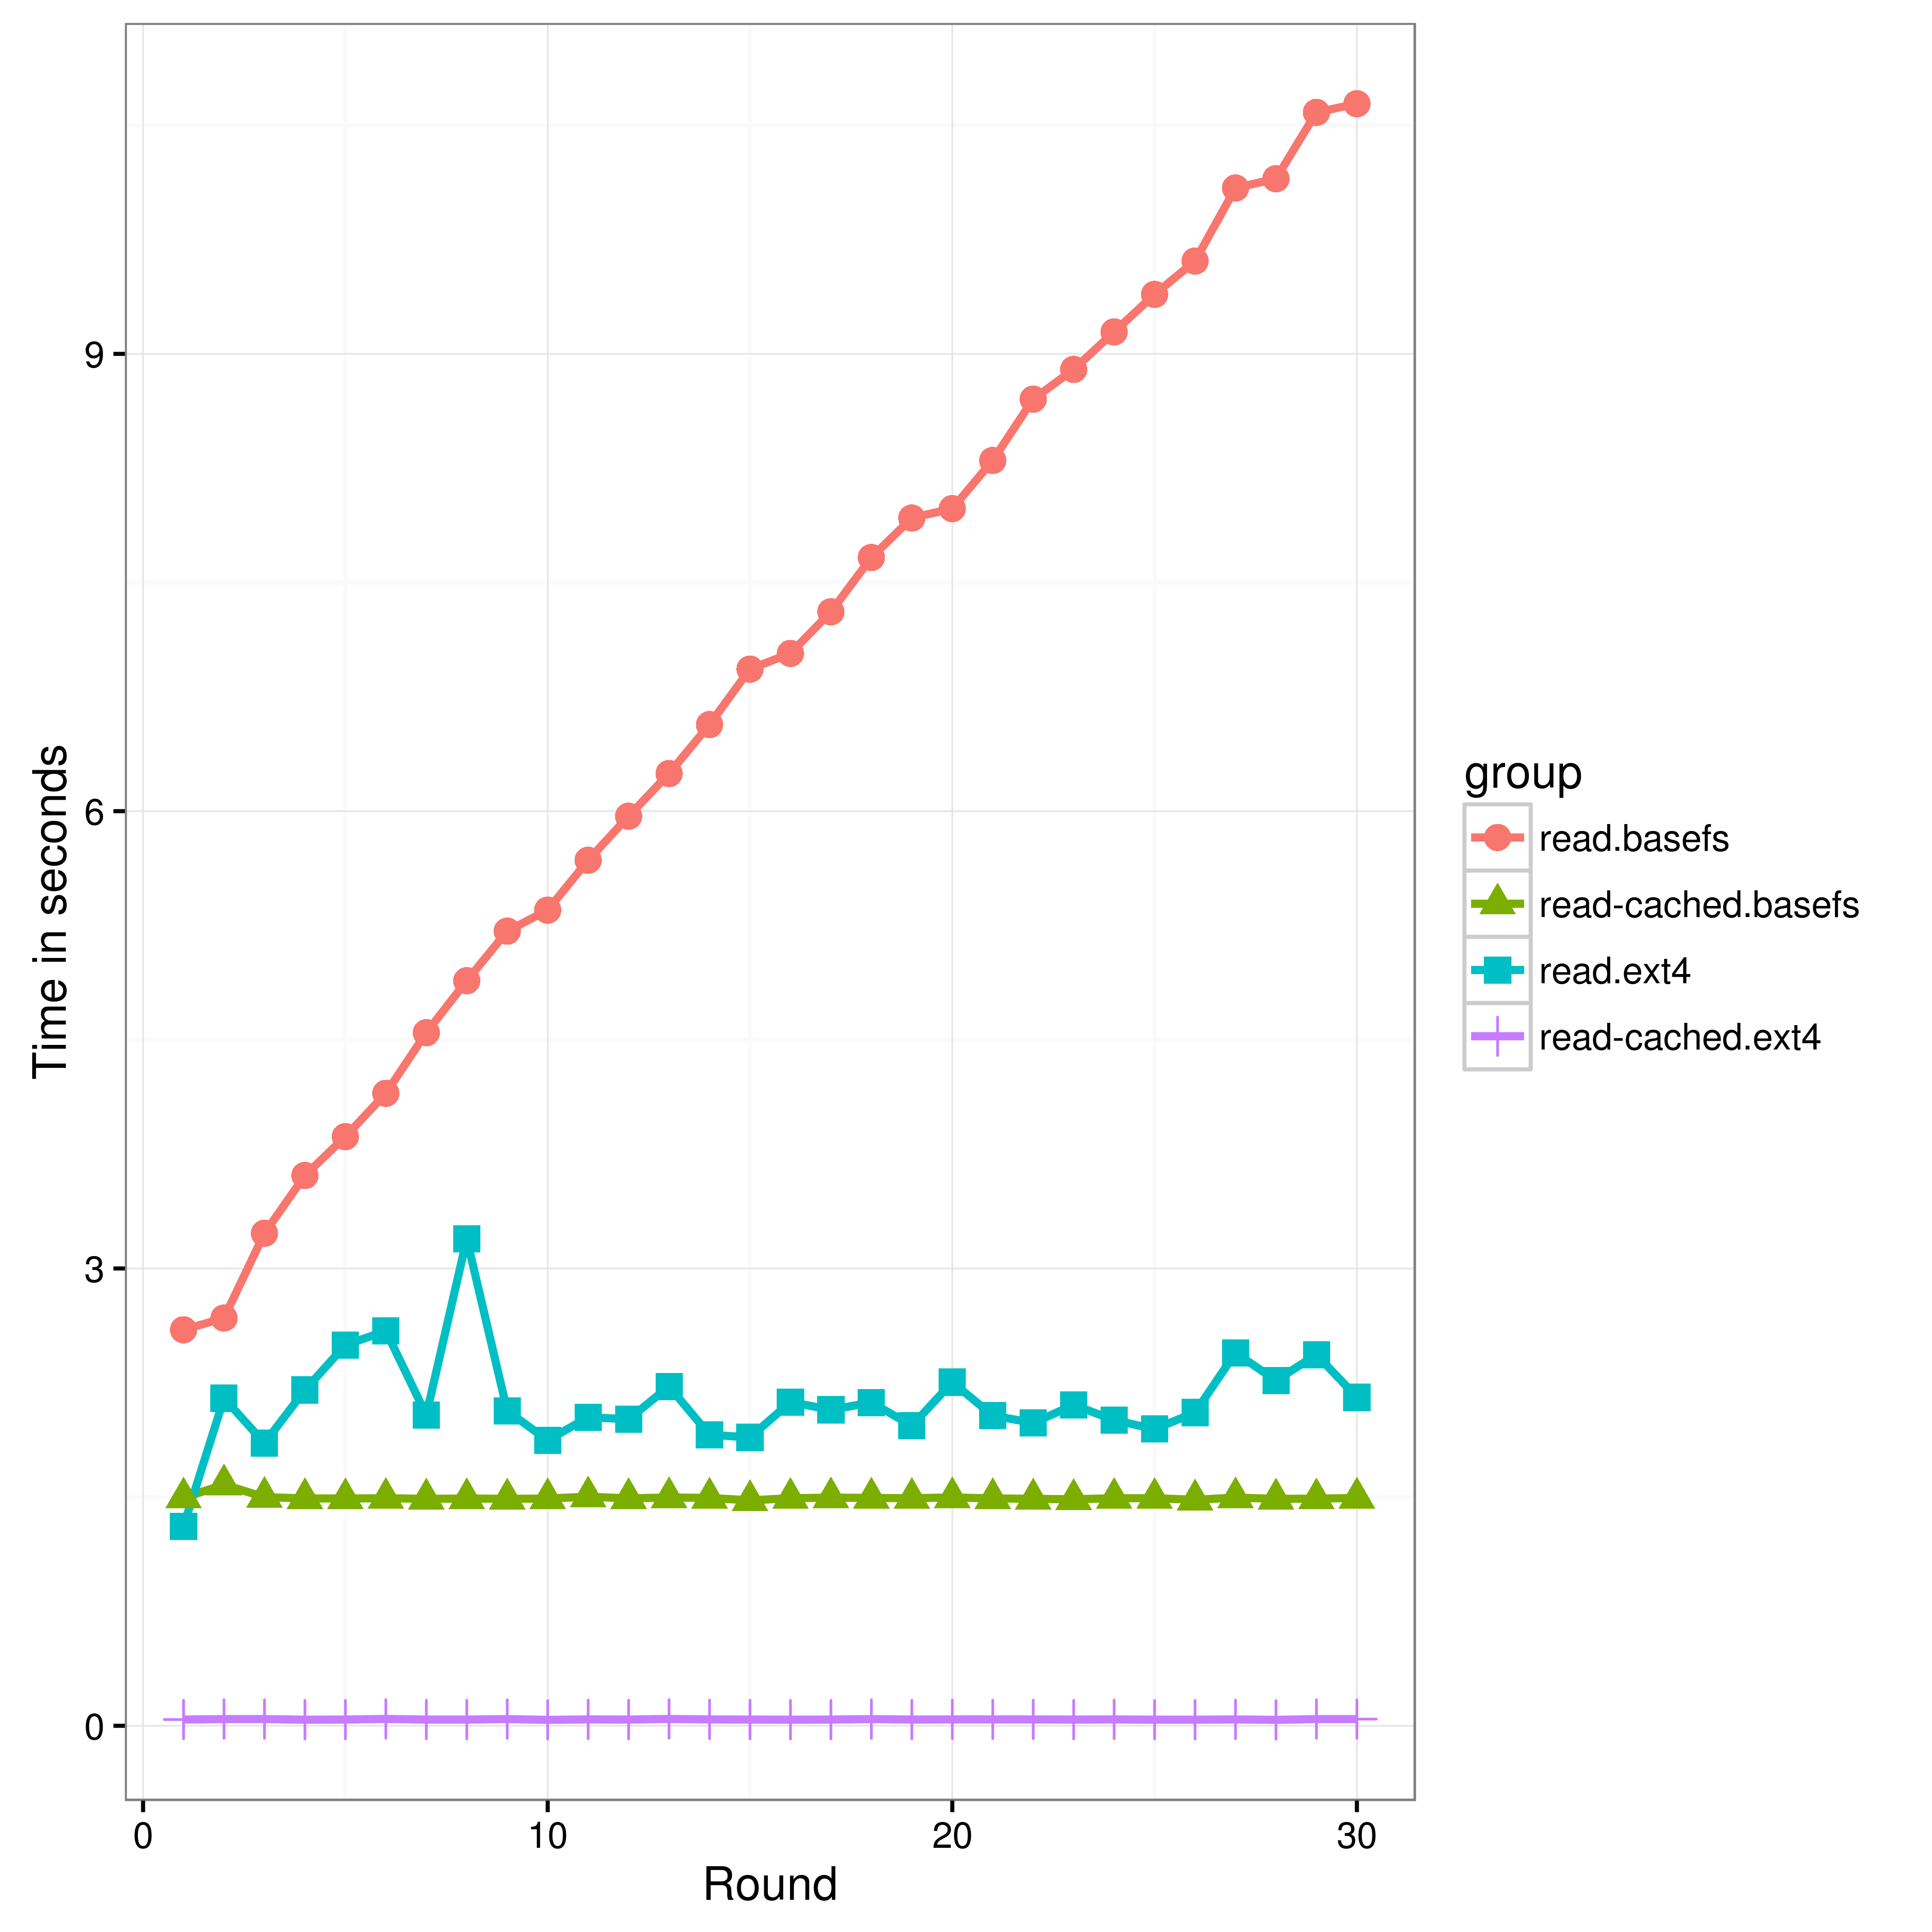
\includegraphics[width=220pt]{imgs/read_performance.png}
\caption{BaseFS vs EXT4 filesystem read performance}
\label{fig:read-performance}
\end{figure}

As expected, cold read performance is linearly affected by the increasing number of patches required to apply for obtaining the most recent version of the content of each configuration file. However, a cached BaseFS reads are faster than uncached EXT4 reads, being able to read the entire filesystem clocking at about 2 seconds.

\subsubsection{Write Performance}


Figure 10 shows how BaseFS write performance compares to EXT4. We can see how in each additional recursive copy of the \texttt{/etc} directory into the BaseFS partition increases the cost consistently. Apart from writing to the log file, BaseFS calculates the binary difference of each file and computes the conflict-free view of the filesystem. This process can be greatly optimized. However, cloud configuration is about changing small bits of information and without a great concern about the performance of massive write operations.


\begin{figure}
\centering
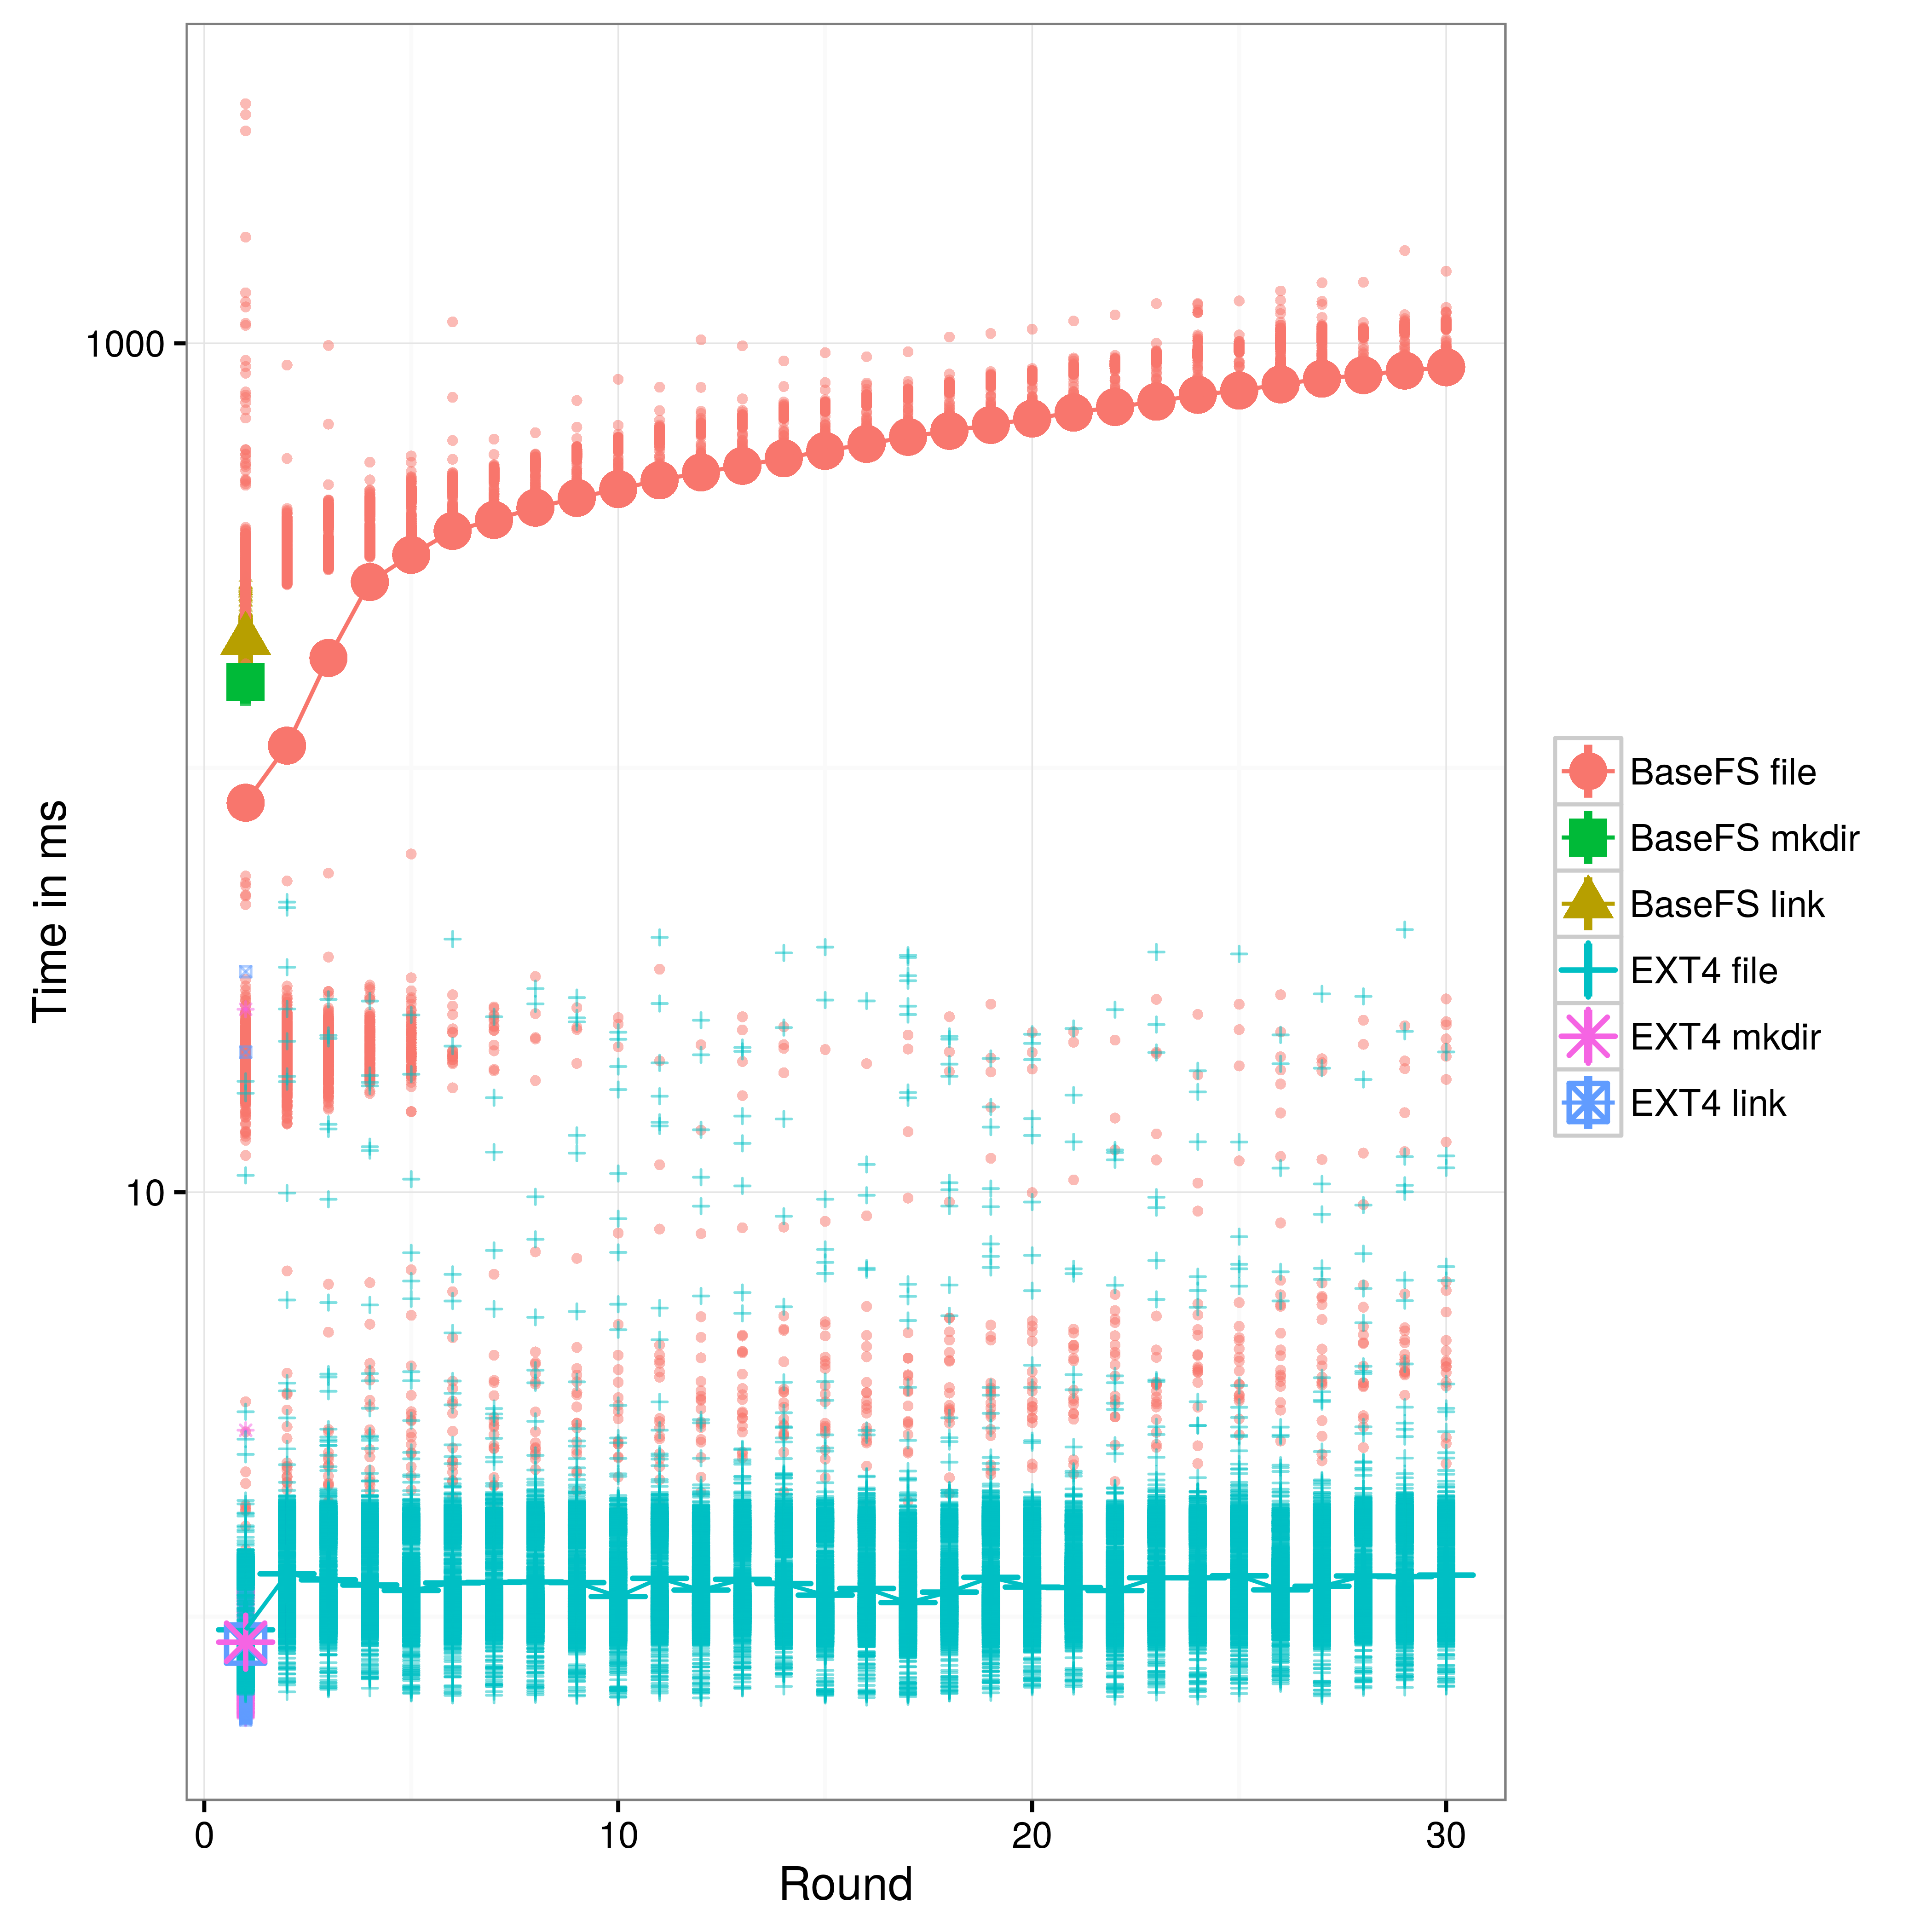
\includegraphics[width=\columnwidth]{imgs/write_performance.png}
\caption{BaseFS vs EXT4 filesystem write performance}
\label{fig:write-performance}
\end{figure}

Cache invalidation is a hard problem to tackle and is effectively limiting what we are able to cache without paying a great cost on implementation complexity. For one, the conflict-free view of the entire filesystem is recomputed on reads that come after 
writes. On the other hand, the file content is also invalidated on a write operation and the binary difference has to be computed using all the BSDIFF4 patches that have been generated since file creation, increasing the cost on each update.

We have made the choice of using BSDIFF4 binary deltas on the grounds that write-intensive workloads are not expected for a cloud configuration tool and a faster convergence time (less messages to gossip) is a more desirable characteristic.


\section{Conclusions and Future Work}

Existing solutions for dynamic configuration, such as etcd, Zookeeper or Consul, are based on strongly consistent and centralized replication. Making them hard to scale, not available under network partitions and complex to operate. For some situations, eventual consistency is sufficient. With this weaker consistency requirements we devise BaseFS, a new replication system that is peer-to-peer, scalable and simple to deploy and operate. Attributes particularly interesting for community cloud environments.

Although current design and implementation has proven effective for cloud configuration, the lack of an existing generalized solution with similar characteristics motivates considering what changes are required to make BaseFS a generalized replication service. BaseFS lack of first-class support for \textbf{large content} is a fundamental problem. Important considerations in this regard are:  
\begin{itemize}
 \item \textbf{Basdiff4 based encoding}. Bsdiff4 is quite memory-hungry, requiring up to $max(17*n,9*n+m)+O(1)$ bytes of memory, where $n$ is the size of the old file and $m$ the size of the new file. \textbf{Multiple encoding methods} should be supported, they can be specified by configuration or perhaps dynamically chosen depending on file characteristics.
 \item \textbf{Hash-linked block list}. Nodes can not know in advance all the block hashes, only the next from the last valid block. An approach that provides the block manifest in advance (figure \ref{fig:infohash}) can make block dissemination more efficient and better tolerant to DDoS attacks. Log entries contain the \textit{roothash}, the root node of a Merkle tree, that expands until their leafs can hold the whole block manifest of a file.
  \item \textbf{Block dissemination}. Blocks are replicated by means of the synchronization protocol. The sync protocol assumes nodes are always willing to cooperate, but as files get bigger more resources are required, encouraging free-riding. An \textbf{incentive mechanism} should be in place in order to discourage non-cooperative behavior. Another issue with the sync protocol is that a node must receive the complete file before being able to perform replication with other nodes. A block exchange protocol like BitSwap, with a \textbf{block-market swarm} is a more effective model of replicating large files.
  \item \textbf{Log unbounded growth}. Deleting log entries is complicated and will required coordinated consensus\cite{letia2009crdts}. However, log entries are not a real concern, they are small and they retain value, as they describe history. What, in some cases, can cause problems are blocks. Block garbage collection can be easily implemented just by removing them from deleted or updated files.
\end{itemize}

\begin{figure}
\centering
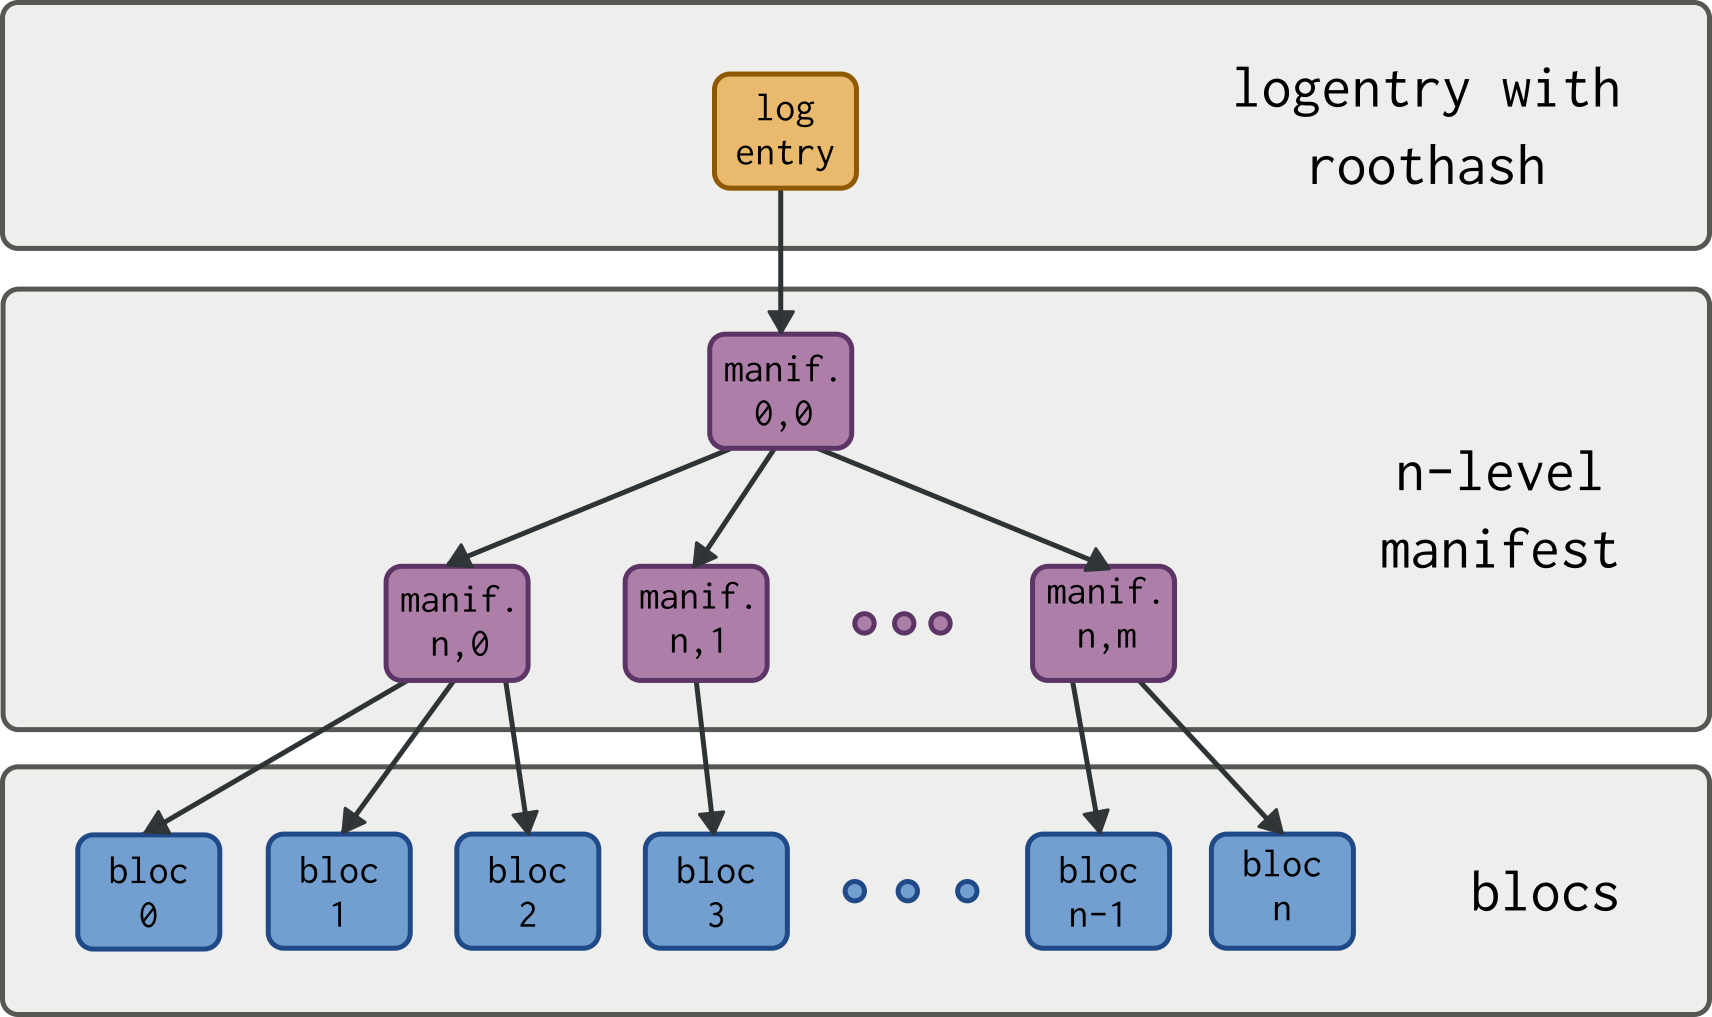
\includegraphics[width=220pt]{imgs/infohash.png}
\caption{Alternative block linking with manifest tree}
\label{fig:infohash}
\end{figure}

% Read permissions is something most systems support, but BaseFS users are expected to encrypt content in advance and perform all PKI management by themselves. Built-in encryption will make privacy requirements less painful.

% BaseFS can take more advantage of the gossip layer. Serf provides network coordinates information that can be used to bias the network communications towards locality. Serf can also provide infrastructure for health checks for monitoring and service discovery, as demonstrated by Consul.

BaseFS model is not limited to cloud configuration, it has the potential of being the foundation for new solutions to distributed replication problems where exiting options require nodes to trust each other. Some of the use cases where our model could be attractive are: Dropbox-like applications, system upgrade on distributed systems, shared in-memory database (memcached), mutable P2P file sharing, live documents like encyclopedia or discography that self-update when new content is available, or distributed version control systems.


\section{Acknowledgments}
The author would like to thank Ester Lopez for her help providing some of the \texttt{R} code for the plots contained in this document.

%
% The following two commands are all you need in the
% initial runs of your .tex file to
% produce the bibliography for the citations in your paper.
\bibliographystyle{abbrv}
\bibliography{sigproc}  % sigproc.bib is the name of the Bibliography in this case
% You must have a proper ".bib" file
%  and remember to run:
% latex bibtex latex latex
% to resolve all references
%
% ACM needs 'a single self-contained file'!
%
%APPENDICES are optional
%\balancecolumns
%\balancecolumns % GM June 2007
% That's all folks!
\end{document}
